% -*- coding: UTF-8 -*-
% vim: autoindent expandtab tabstop=4 sw=4 sts=4 filetype=tex
% chktex-file 27 - disable warning about missing include files

% Main document
% ===========================================================================
% This is part of the document "Project documentation template".
% Authors: brd3, kaa1
%
%---------------------------------------------------------------------------

\documentclass[
    a4paper,      % paper format
    10pt,         % fontsize
    %twoside,     % double-sided
    openright,    % begin new chapter on right side
    notitlepage,  % use no standard title page
    parskip=half, % set paragraph skip to half of a line
]{scrreprt}       % KOMA-script report
%---------------------------------------------------------------------------
\raggedbottom{}
\KOMAoptions{cleardoublepage=plain} % Add header and footer on blank pages

% Load Standard Packages:
%---------------------------------------------------------------------------
\usepackage{scrpage2}                    % Control of page headers and footers in LaTeX,
                                         % needed for e.g. deftripstyle (to defined page styles)
\usepackage[ngerman]{babel}              % german hyphenation
\usepackage[utf8]{inputenc}              % UTF-8 input encoding
\usepackage[T1]{fontenc}                 % hyphenation of words with ä,ö and ü
\usepackage{textcomp}                    % additional symbols
\usepackage{float}                       % floating objects
\usepackage{booktabs}                    % package for nicer tables
\usepackage{tocvsec2}                    % provides means of controlling the sectional numbering
\usepackage{pgfgantt}                    % Provides GANTT charts
\usepackage[owncaptions]{vhistory}       % Provides framework for creating history outline
\renewcommand{\vhhistoryname}{Versionen} % Rename version history to german name "Versionen"
\usepackage{csquotes}                    % Quotes
\usepackage{nameref}                     % Allows referencing of names
\usepackage{tabu}                        % Long table is long
%---------------------------------------------------------------------------

%---------------------------------------------------------------------------
\usepackage{enumitem}                    % Allows multiple types of enumerations
\newlist{longenum}{enumerate}{5}
\setlist[longenum,1]{label=\roman*)}  % chktex 9: solo } found -- chktex 10: expected ) found }
\setlist[longenum,2]{label=\alph*)}   % chktex 9 chktex 10
\setlist[longenum,3]{label=\arabic*)} % chktex 9 chktex 10
\setlist[longenum,4]{label=(\roman*)} % chktex 9 chktex 10 chktex 36: put space in front of parenthesis
\setlist[longenum,5]{label=(\alph*)}  % chktex 9 chktex 10 chktex 36
%---------------------------------------------------------------------------

% Bibliography
%---------------------------------------------------------------------------
% \usepackage[
%     style=alphabetic,
%     backend=biber,
%     citestyle=authoryear
% ]{biblatex}
% \addbibresource{inc/static/bibliography.bib}
\usepackage[
    backend=biber,
    style=ieee,
    sortlocale=de_DE,
    natbib=true,
    url=false, 
    doi=true,
    eprint=false
]{biblatex}
% \bibliographystyle{IEEEtranS}
\addbibresource{inc/static/bibliography.bib}
\DefineBibliographyStrings{ngerman}{
    andothers = {{et\,al\adddot}},
}
%---------------------------------------------------------------------------

% Load Math Packages
%---------------------------------------------------------------------------
\usepackage{mathtools}                       % Provide equation and gather environments
\usepackage{amsthm}                          % Provide the possibility to define definitions
\theoremstyle{definition}                    % Add new theorem style
\newtheorem{definition}{Definition}[section] % Add new theorem
\usepackage{bm}                              % bold font in math mode
\usepackage{amssymb}                         % mathematical special characters, e.g. mathbb
\usepackage{exscale}                         % mathematical size corresponds to textsize
\usepackage{esvect}                          % Provides nicer vector display in math mode
%---------------------------------------------------------------------------

% Definition of fonts
%---------------------------------------------------------------------------
\DeclareFixedFont{\ttb}{T1}{txtt}{bx}{n}{9} % for bold
\DeclareFixedFont{\ttm}{T1}{txtt}{m}{n}{9}  % for normal
%---------------------------------------------------------------------------

% Definition of colors
%---------------------------------------------------------------------------
\RequirePackage{color}
\definecolor{linkblue}{rgb}{0,0,0.8}       % Standard
\definecolor{darkblue}{rgb}{0,0.08,0.45}   % Dark blue
\definecolor{bfhgrey}{rgb}{0.41,0.49,0.57} % BFH grey
\definecolor{linkcolor}{rgb}{0,0,0}
\colorlet{Black}{black}
\definecolor{keywords}{rgb}{255,0,0}
\definecolor{red}{rgb}{0.6,0,0}
\definecolor{green}{rgb}{0,0.5,0}
\definecolor{blue}{rgb}{0,0,0.5}
% Syntax colors
\definecolor{syntaxRed}{rgb}{0.6,0,0}
\definecolor{syntaxBlue}{rgb}{0,0,0.5}
\definecolor{syntaxComment}{rgb}{0,0.5,0}
% Background colors
\definecolor{syntaxBackground}{rgb}{0.95, 0.95, 0.95}
%---------------------------------------------------------------------------

% Embed graphics
%---------------------------------------------------------------------------
\usepackage{graphicx}                    % Allows embedding of images
\newcommand*{\img}[2][\baselineskip]{%
    \raisebox{-.3\baselineskip}{%
        \includegraphics[
        height={#1},
        width={#1},
        keepaspectratio,
        ]{#2}%
    }%
}
%---------------------------------------------------------------------------

% Load listing package
% which produces formatted program listings
%---------------------------------------------------------------------------
\usepackage{listing}
\renewcommand{\listingname}{Auflistung}
%---------------------------------------------------------------------------

% Load listings package
% which provides source code formatting
%---------------------------------------------------------------------------
\usepackage{listings}
% Change captions of listings
\renewcommand{\lstlistingname}{Auflistung}
\renewcommand{\lstlistlistingname}{Auflistungsverzeichnis}
\usepackage{glslListings}
% Make sure Umlauts are getting displayed correctly.
\lstset{literate=%
    {Ö}{\textcolor{black}{\"O}}1
    {Ä}{{\"A}}1
    {Ü}{{\"U}}1
    {ß}{{\ss}}1
    {ü}{{\"u}}1
    {ä}{{\textcolor{black}{\"a}}}1
    {ö}{{\textcolor{black}{\"o}}}1
    {~}{{\textasciitilde}}1
    {?}{{\textcolor{black}{?}}}1
}
% Define a list style for Python programming language
\lstset{language=Python,
    basicstyle=\ttm\ttfamily\linespread{1.15},
    backgroundcolor = \color{syntaxBackground},
    columns=fullflexible,
    commentstyle=\color{green},
    emphstyle=\ttb\color{red},
    escapechar=§,
    frame=tlbr,
    framesep=0.2cm,
    framerule=0pt,
    numbers=left,
    numbersep=5pt,                   % how far the line-numbers are from the code
    numberstyle=\tiny\color{gray}, % the style that is used for the line-numbers
    identifierstyle=\color{black},
    keywordstyle=\ttb\color{blue},
    otherkeywords={self},
    % procnamekeys={def,class},
    showspaces=false,
    showstringspaces=false,
    showtabs=false,
    tab=\rightarrowfill,
    xleftmargin=0.7cm,
}
%---------------------------------------------------------------------------

% Hyperref Package (Create links in a pdf)
%---------------------------------------------------------------------------
\usepackage[
    pdftex,ngerman,bookmarks,plainpages=false,pdfpagelabels,
    backref = {false},                                        % No index backreference
    colorlinks = {true},                                      % Color links in a PDF
    hypertexnames = {true},                                   % no failures "same page(i)"
    bookmarksopen = {true},                                   % opens the bar on the left side
    bookmarksopenlevel = {0},                                 % depth of opened bookmarks
    pdftitle = {Volume ray casting --- basics \& principles}, % PDF-property
    pdfauthor = {Sven Osterwalder},                           % PDF-property
    pdfsubject = {Volume ray casting},                        % PDF-property
    linkcolor = {linkcolor},                                  % Color of Links
    citecolor = {linkcolor},                                  % Color of Cite-Links
    urlcolor = {linkcolor},                                   % Color of URLs
]{hyperref}
%---------------------------------------------------------------------------

% Geometry package: Set up page dimension
%---------------------------------------------------------------------------
\usepackage[a4paper,
    left=25mm,
    right=25mm,
    top=27mm,
    headheight=20mm,
    headsep=10mm,
    textheight=242mm,
    footskip=15mm
]{geometry}
%---------------------------------------------------------------------------

% Makeindex Package
%---------------------------------------------------------------------------
\usepackage{makeidx}
\makeindex
%---------------------------------------------------------------------------

% Glossary Package
%---------------------------------------------------------------------------
\usepackage[nonumberlist,nomain]{glossaries}
% -*- coding: UTF-8 -*-
% vim: autoindent expandtab tabstop=4 sw=4 sts=4 filetype=tex
% chktex-file 27


\makeglossaries{}
%---------------------------------------------------------------------------

% Fancyrb package
%---------------------------------------------------------------------------
\usepackage{fancyvrb}
\RecustomVerbatimCommand{\VerbatimInput}{VerbatimInput}
{fontsize=\footnotesize,
    frame=lines,  % top and bottom rule only
    framesep=2em, % separation between frame and text rulecolor=\color{Gray},
    label=\fbox{\color{Black}},
    labelposition=topline,
    % commandchars=\|\(\), % escape character and argument delimiters for
    % commands within the verbatim
    % commentchar=*        % comment character
}
%---------------------------------------------------------------------------

% TODO notes package
%---------------------------------------------------------------------------
\usepackage[textwidth=65mm]{todonotes}
%---------------------------------------------------------------------------

\begin{document}
\settocdepth{section}
\pagenumbering{roman}

% Document title
%---------------------------------------------------------------------------
\providecommand{\titel}{QDE --- a visual animation system.}
%---------------------------------------------------------------------------

% Set up header and footer using page style
%---------------------------------------------------------------------------
\deftripstyle{newlayout}
  [0pt] % no header line
  [0pt] % no footer line
  {} % Header left
  {} % Header center
  {} % Header right
  {\color{bfhgrey} \footnotesize \titel, Version \vhCurrentVersion,
      \vhCurrentDate} % Footer left
  {} % Footer center
  {\color{bfhgrey} \thepage} % Footer right

\deftripstyle{titlepageStyle}
  [0pt] % no header line
  [0pt] % no footer line
  {} % Header left
  {} % Header center
  {} % Header right
  {\color{bfhgrey}\fontsize{9pt}{10pt}\selectfont
    Berner Fachhochschule | Haute école spécialisée bernoise | Bern
    University of Applied Sciences} % Footer left
  {} % Footer center
  {} % Footer right


\pagestyle{newlayout}
% use "pagestyle" also on chapter starting pages
\renewcommand{\chapterpagestyle}{newlayout}
\renewcommand{\chaptermark}[1]{\markboth{\thechapter.  #1}{}}
\renewcommand*{\headfont}{\normalfont}
\renewcommand*{\footfont}{\normalfont}
%---------------------------------------------------------------------------

% Title Page and Abstract
%---------------------------------------------------------------------------
\setcounter{page}{1}
% -*- coding: UTF-8 -*-
% vim: autoindent expandtab tabstop=4 sw=4 sts=4 filetype=tex
% chktex-file 27 - disable warning about missing include files
% chktex-file 36 - disable put space in front of parentheses warning

\begin{titlepage}

    % BFH-Logo absolute placed at (28,12) on A4 and picture (16:9 or 15cm x 8.5cm)
    % Actually not a realy satisfactory solution but working.
    %---------------------------------------------------------------------------
    \setlength{\unitlength}{1mm}
    
\includegraphics[scale=1.0]{img/BFH_Logo_B}

    \begin{picture}(150,2)
        \put(0,0){\color{bfhgrey}\rule{150mm}{2mm}}
    \end{picture}

    \begin{figure}[H]
        \hspace*{0.25cm}
        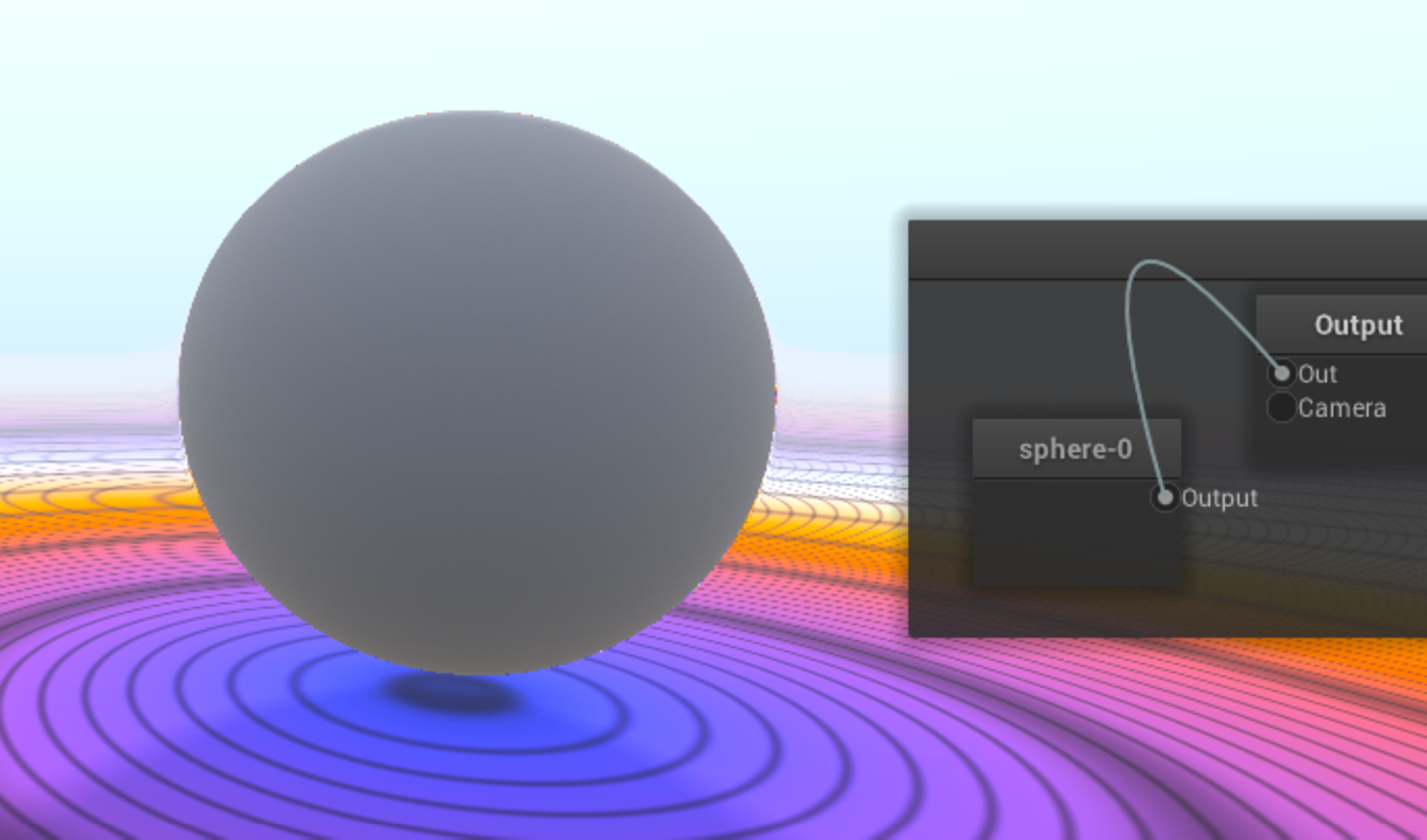
\includegraphics{img/logo.pdf}
    \end{figure}

    \begin{picture}(150,2)
        \put(0,0){\color{bfhgrey}\rule{150mm}{2mm}}
    \end{picture}

    \begin{flushleft}
        \fontsize{26pt}{28pt}\selectfont
        \titel{}\\
        \vspace{3mm}
        \textbf{A visual animation system} \\
        \vspace{6mm}
        \fontsize{14pt}{16pt}\selectfont
        \textbf{MTE7102: Projektarbeit 2} \\
        \vspace{3mm}

        \fontsize{10pt}{17pt}\selectfont
        \begin{tabbing}
        xxxxxxxxxxxxxxx   \= xxxxxxxxxxxxxxxxxxxxxxxxxxxxxxxxxxxxxxxxxxxxxxx \kill
        Studiengang:      \> Informatik                                         \\
        Autor:            \> Sven Osterwalder\protect\footnotemark[1]{}         \\
        Betreuer:         \> Prof.~Claude Fuhrer\protect\footnotemark[2]{} \\
        Datum:            \> \vhCurrentDate{}\\
        Version:          \> \vhCurrentVersion\\
        \end{tabbing}
    \end{flushleft}
    \footnotetext[1]{sven.osterwalder@students.bfh.ch}
    \footnotetext[2]{claude.fuhrer@bfh.ch}

    \vfill
    
\includegraphics[height=\baselineskip]{img/by-sa}\\ \small{\sffamily{Licensed under the Creative Commons Attribution-ShareAlike 3.0 License}}

    \thispagestyle{titlepageStyle}

\end{titlepage}

% -*- coding: UTF-8 -*-
% vim: autoindent expandtab tabstop=4 sw=4 sts=4 filetype=tex
% chktex-file 27 - disable warning about missing include files

% Versionenkontrolle :
% -----------------------------------------------

\chapter*{}
\label{chap:versionen}

\begin{versionhistory}
    \vhEntry{0.1}{24.07.2016}{SO}{Initiale Erstellung des Dokumentes}
\end{versionhistory}

\listoftodos{}
\addcontentsline{toc}{chapter}{Abstract}
% -*- coding: UTF-8 -*-
% vim: autoindent expandtab tabstop=4 sw=4 sts=4 filetype=tex
% chktex-file 27

\chapter*{Abstract}
\label{chap:abstract}

Diese Projektarbeit stellt eine Software-Architektur für ein System zur
einfachen Erstellung und Handhabung visueller Szenen in Echtzeit vor.

Das System erlaubt die Erstellung und Handhabung von Szenen mittels einer
grafischen Benutzeroberfläche (GUI). Ein Graph erlaubt eine einfache und
intuitive Komposition von visuellen Szenen. Ein Sequenzer erlaubt die Animation
von Elementen, wie z.B. Modellen oder Bitmaps.

Als Renderingverfahren kommt Sphere Tracing zum Einsatz, ein hoch-optimiertes
Ray-Tracing-Verfahren, welches die Darstellung von Szenen in Echtzeit per GPU
erlaubt.

Die Machbarkeit des Konzeptes wird durch einen Prototypen aufgezeigt, welcher
die Komposition sowie Darstellung von einfachen Szenen in Echtzeit erlaubt.

%---------------------------------------------------------------------------

% Table of contents
%---------------------------------------------------------------------------
\tableofcontents
\cleardoublepage{}
%---------------------------------------------------------------------------

% Main part:
%---------------------------------------------------------------------------
\pagenumbering{arabic}
% -*- coding: UTF-8 -*-
% vim: autoindent expandtab tabstop=4 sw=4 sts=4 filetype=tex
% vim: spelllang=de
% chktex-file 27 - disable warning about missing include files

\chapter{Einleitung}
\label{chap:10_introduction}

In~\cite{osterwalder_sven_volume_2016} wurde mit Sphere-Tracing ein hoch
effizientes Ray-Tracing-Verfahren vorgestellt, welches Objekte (und somit auch
Szenen) sowie Operationen mittels impliziten Funktionen darstellt. Dies mag auf
den ersten Blick praktisch erscheinen, da die Definition der meisten Objekte
und Operationen nur wenige Zeilen lang ist. Dies hat jedoch zur Folge, dass
einerseits Programme selbst bei kleinsten Änderungen neu kompiliert werden
müssen und, dass andererseits bei komplexen Szenen schnell die Übersicht
verloren geht. Möchte man Szenen beziehungsweise Objekte animieren, so erhöht
dies die Komplexität erneut.

Diese Projektarbeit stellt daher eine Software-Architektur für ein System zur
einfachen Erstellung und Handhabung visueller Szenen in Echtzeit vor.

Das System erlaubt die Erstellung und Handhabung von Szenen mittels einer
grafischen Benutzeroberfläche (GUI). Ein Graph erlaubt eine einfache und
intuitive Komposition von visuellen Szenen. Ein Sequenzer erlaubt die Animation
von Elementen, wie z.B. Modellen oder Bitmaps.

Als Renderingverfahren kommt Sphere-Tracing
zum Einsatz, ein hoch-optimiertes Ray-Tracing-Verfahren, welches die
Darstellung von Szenen in Echtzeit per GPU erlaubt.

Die Machbarkeit des Konzeptes wird durch einen Prototypen aufgezeigt, welcher
die Komposition sowie Darstellung von einfachen Szenen in Echtzeit erlaubt.

%* -*- coding: UTF-8 -*-
% vim: autoindent expandtab tabstop=4 sw=4 sts=4 filetype=tex
% vim: spelllang=de spell
% chktex-file 27 - disable warning about missing include files

\chapter{Administratives}
\label{chap:20_administrative}

Einige administrative Aspekte der Projektarbeit werden angesprochen,
obwohl sie für das Verständnis der Resultate nicht notwendig sind.

Im gesamten Dokument wird nur die männliche Form verwendet, womit aber
beide Geschlechter gemeint sind.

\section{Beteiligte Personen}
\label{sec:involved_persons}

\begin{tabbing} %tabulator
Bezeichnung: \= Name name name name name name\= Zuständigkeit \kill \\
    Autor           \> Sven Osterwalder\protect\footnotemark[1]{}    \> \\
    Betreuer        \> Prof.\ Claude Fuhrer\protect\footnotemark[2]{}  \> \textit{Begleitet den Studenten bei der Projektarbeit}\\
\end{tabbing}
\footnotetext[1]{sven.osterwalder@students.bfh.ch}
\footnotetext[2]{claude.fuhrer@bfh.ch}

\section{Aufbau des Dokumentes}
\label{sec:document_structure}

Die vorliegende Arbeit ist aufgebaut wie folgt:
\begin{itemize}
    \item Einleitung zur Projektarbeit
    \item Beschreibung der Aufgabenstellung
    \item Vorgehen des Autors im Hinblick auf die gestellten Aufgaben
    \item Lösung der gestellten Aufgaben
    \item Verwendete Technologien
\end{itemize}

\section{Ergebnisse (Deliverables)}
\label{sec:deliverables}

Nachfolgend sind die abzugebenden Objekte aufgeführt:
\begin{itemize}
    \item \textbf{Abschlussdokument} \\
        Das Abschlussdokument beinhaltet die Ausarbeitung einer
        Software-Architektur eines Systems zur einfachen Erstellung und
        Handhabung visueller Szenen in Echtzeit.
    \item \textbf{Protoyp} \\
        Der~\hyperref[chap:prototype]{Prototyp} entstand im Rahmen der
        Bearbeitung der Thematik. Er zeigt die Machbarkeit (von Teilen) der
        angedachten Software-Architektur auf.
\end{itemize}

% -*- coding: UTF-8 -*-
% vim: autoindent expandtab tabstop=4 sw=4 sts=4 filetype=tex
% vim: spelllang=de spell
% chktex-file 27 - disable warning about missing include files

\chapter{Aufgabenstellung}
\label{chap:scope}

\section{Motivation}
\label{sec:motivation}

Das in der vorhergehenden
Projektarbeit~\cite{osterwalder_sven_volume_2016} vorgestellte
Renderingverfahren, Sphere Tracing, optimiert das \todo{write ray tracing everywhere
    the same way} Raytracing-Verfahren so weit, dass eine Darstellung von
Szenen mit hoher Qualität in Echtzeit möglich ist.

Das Verfahren nutzt implizite Funktionen um Objekte (und somit auch
Szenen) zu definieren. Selbiges gilt auch für Operationen. Dies mag auf
den ersten Blick praktisch erscheinen, da die Definitionen der meisten Objekte
und Operationen nur wenige Zeilen lang sind. Dies hat jedoch zur Folge, dass
einerseits Programme selbst bei kleinsten Änderungen neu kompiliert werden
müssen und, dass andererseits bei komplexen Szenen schnell die Übersicht
verloren geht. Möchte man Szenen bzw.\ Objekte animieren, so erhöht dies die
Komplexität erneut.

Diese Projektarbeit stellt daher eine Software-Architektur für ein System zur
einfachen Erstellung und Handhabung visueller Szenen in Echtzeit vor.

Die Machbarkeit des \todo{check if Konzept is the right word} Konzeptes wird
durch einen Prototypen aufgezeigt, welcher die Komposition sowie Darstellung
von einfachen Szenen in Echtzeit erlaubt.

\subsection{Demoszene}
\label{subsec:demoscene}

In den 1980er-Jahren entwickelte sich ``unter Anhängern der
Computerszene \dots{} während der Blütezeit der
8-Bit-Systeme''~\parencite{wikipedia_foundation_demoszene_2015} eine Bewegung
namens Demoszene. ``Ihre Mitglieder, die häufig Demoszener oder einfach
Szener genannt werden, erzeugen mit Computerprogrammen auf Rechnern so
genannte Demos – Digitale Kunst, meist in Form von musikalisch
unterlegten
Echtzeit-Animationen.''~\parencite{wikipedia_foundation_demoszene_2015}

Es handelt sich bei der Demoszene um ein sehr aktives und kreatives
Umfeld, in welchem die Technologie ständig an die Grenzen ihrer
Möglichkeiten gebracht wird. In diesem Umfeld entstehen regelmässig neue
Ideen zur Erzeugung von noch realistischer wirkenden Bildern. Dabei
findet eine wechselseitige Beeinflussung zwischen dem akademischen
Umfeld und der Demoszene statt.

So wurde auch das in~\cite{osterwalder_sven_volume_2016} vorgestellte
\textit{Sphere Tracing} Verfahren
relativ früh von in der Demoszene aktiven Personen aufgegriffen und
behandelt.

\section{Ziele und Abgrenzung}
\label{sec:objectives}

Diese Projektarbeit besteht aus zwei Teilen. Der Beschreibung der \todo{add
    ref.\ to sw.\ arch.\ chapter} Software-Architektur sowie der Umsetzung
eines~\hyperref[chap:prototype]{Prototypen}. \todo{Explain, that prototype was
    done before}Dieser bildet einen kleinen Teil
der Software-Architektur ab.

Bei dem entwickelten~\hyperref[chap:prototype]{Prototypen} handelt es sich um
eine Machbarkeitsstudie. Diese zeigt, dass die Komposition sowie Darstellung
von einfachen Szenen in Echtzeit mit dem angedachten System möglich ist.

Diese Projektarbeit dient als Vorarbeit und Grundlage für das MSE-Modul
\textit{MTE7103} --- ``Master Thesis'' (Folgemodul und Abschlussarbeit).

\subsection{Vorgängige Aktivitäten}
\label{subsec:preliminaries}

Die vorhergehende Projektarbeit~\cite{osterwalder_sven_volume_2016} bildet die
Grundlage für diese Projektarbeit.

\subsection{Neue Lerninhalte}
\label{subsec:new_learning_contents}

Zusätzlich zu den formalen Lerninhalten hatte die Arbeit für den Autor
die folgenden \todo{Provide new learning contents} neuen Lerninhalte:
\begin{itemize}
    \item{TODO}
\end{itemize}

% -*- coding: UTF-8 -*-
% vim: autoindent expandtab tabstop=4 sw=4 sts=4 filetype=tex
% vim: spelllang=de spell
% chktex-file 27 - disable warning about missing include files

\chapter{Vorgehen}
\label{chap:procedure}

\section{Arbeitsorganisation}
\label{sec:organization}

\subsection{Treffen}
\label{subsec:meetings}

Besprechungen mit dem Betreuer der Arbeit halfen, die gesteckten Ziele zu
erreichen und Fehlentwicklungen zu vermeiden. Der Betreuer unterstützte den
Autor dabei mit Vorschlägen. Insgesamt fanden vier Treffen statt. Sie wurden in
Form eines Protokolles festgehalten. Das Protokoll findet sich
unter~\autoref{chap:10_meeting_minutes}.

\section{Projektphasen}
\label{sec:project_schedule}

\subsection{Meilensteine}
\label{subsec:milestones}

Um bei der Arbeit ein möglichst strukturiertes Vorgehen einzuhalten,
wurden folgende Projektphasen gewählt:

\begin{itemize}
    \item Start der Projektarbeit
    \item Erarbeitung und Festhalten der Anforderungen
    \item Erstellung eines~\hyperref[chap:prototype]{Prototypen}
    \item Erstellung der abschliessenden Dokumentation aufgrund der gewonnen
        Erkenntnisse
\end{itemize}

Die Phasen \textit{Erstellung eines Prototypen} sowie\textit{Erstellung der
    abschliessenden Dokumentation}liefen parallel ab. Erkenntnisse einer Phase
flossen jeweils in die andere Phase ein.

\subsection{Zeitplan / Projektphasen}
\label{subsec:timeschedule}

\begin{figure}[H]
    \begin{ganttchart}[
        vgrid,
        x unit=0.43cm,
        bar/.append style={fill=bfhgrey!50},
    ]{1}{25}
        \gantttitle{2016}{25} \ganttnewline{}
        \gantttitlelist{8,...,32}{1} \ganttnewline{} % chktex 11: Disable "you should use \ldots to achieve.."
        \ganttbar{Projektstart}{1}{1} \ganttnewline{}
        \ganttlinkedbar{Anforderungen}{2}{3} \ganttnewline{}
        \ganttlinkedbar{Erstellung Prototyp}{4}{10} \ganttnewline{}
        \ganttlinkedbar{Dokumentation}{14}{23} \ganttnewline{}
        \ganttlinkedbar{Korrekturen}{23}{24} \ganttnewline{}
        \ganttlinkedmilestone{Abgabe Dokumentation}{24} \ganttnewline{}
        \ganttbar{Erstellung Prototyp}{23}{23} \ganttnewline{}
        \ganttbar{Vorbereitung Präsentation/Verteidigung}{24}{25} \ganttnewline{}
        \ganttmilestone{Präsentation/Verteidigung}{25}
    \end{ganttchart}
    \caption{Zeitplan; Der Titel stellt Jahreszahlen, der Untertitel
    Kalenderwochen dar}\label{fig:timeschedule}
\end{figure}

\subsubsection{Projektstart}
\label{subsubsec:kick_off}

In der ersten Phase wurden die Zwischenziele der Arbeit identifiziert
und skizziert.

\subsubsection{Anforderungen}
\label{ssubsec:requirements}

In dieser Phase wurde das Ziel dieser Projektarbeit festgelegt.
Ausgehend vom Ziel wurden die dazu erforderlichen Projektphasen
festgelegt.

\subsubsection{Erstellung Prototyp}
\label{ssubsec:prototype}

Ausgehend von den Anforderungen und vor allem der Vision, wurde ein Prototyp
erstellt um die Machbarkeit aufzuzeigen und um Erkenntnisse zu gewinnen.

\subsubsection{Dokumentation}
\label{ssubsec:documentation}

Die vorliegende Arbeit entspricht der Dokumentation. Sie sollte während der
gesamten Projektarbeit stetig erweitert werden. Allerdings wurde zu viel Fokus
auf den Prototypen gelegt und somit wurde die Dokumentation eher erst spät
richtig angegangen. Sie diente zur Reflexion von fertiggestellten Teilen.

\section{Technologien}
\label{sec:technologies}

\subsection{Tools und Software}
\label{subsec:tools_software}

\subsubsection{Dokumentation und Prototyp}
\label{ssubsec:tools_software:documentation_prototype}

\begin{description}
    \item[\LaTeX] Eine Makro-Sammlung für das \TeX-System. Wurde zur
        Erstellung dieser Dokumentation eingesetzt. Diese Dokumentation
        wurde mittels \LaTeX{} geschrieben.
    \item[Make] Build-Automations-Werkzeug, wurde zur Erstellung dieses Dokumentes eingesetzt.
    \item[CMake] Build-Automations-Werkzeug, wurde zur Erstellung des
        \hyperref[chap:prototype]{Prototypen} eingesetzt.
    \item[zotero] Ein freies, quelloffenes Literaturverwaltungsprogramm
        zum Sammeln, Verwalten und Zitieren unterschiedlicher Online-
        und Offline-Quellen~\parencite{wikipedia_foundation_zotero_2015}.
    \item[VIM] Vi IMproved. Ein freier, quelloffener Texteditor zur
        Textbearbeitung. Er wurde zum Verfassen der Dokumentation sowie zur
        Entwicklung des~\hyperref[chap:prototype]{Prototypen} eingesetzt.
    \item[LLVM] Low Level Virtual Machine. Eine Compiler-Architektur zum
        Kompilieren von Applikationen. Wurde zur Kompilation des
        \hyperref[chap:prototype]{Prototypen} eingesetzt.
    \item[clang] Ein C-Sprachen-Frontend für LLVM.\ Wurde zur Kompilation
        des~\hyperref[chap:prototype]{Prototypen} eingesetzt.
    \item[Papyrus] Ein quelloffenes Werkzeug zur Erstellung von UML- und
        SysML-Modellen~\parencite{the_eclipse_foundation_papyrus_2015}.
    \item[Pencil] Ein quelloffenes Werkzeug zur Erstellung von Prototypen von
        grafischen Benutzeroberflächen~\parencite{evolus_pencil_2015}.
\end{description}


\subsubsection{Arbeitsorganisation}
\label{ssubsec:tools_software:job_organisation}

\begin{description}
    \item[Git] Freie Software zur verteilten Versionsverwaltung, wurde
        für die Entwicklung dieser Dokumentation sowie
        des~\hyperref[chap:prototype]{Prototypen} verwendet. Die
        Projektarbeit findet sich
        unter~\href{https://www.github.com/sosterwalder/mte7101-project1}{GitHub}\footnote{
        \href{https://www.github.com/sosterwalder/mte7101-project1}{https://www.github.com/sosterwalder/mte7101-project1}
    }.
    \item[GitHub] Eine freie Hosting-Platform für Git mit Weboberfläche.
\end{description}

\subsection{Standards und Richtlinien}
\label{subsec:standards_guidelines}

\subsubsection{Programmcode}
\label{ssubsec:standards_guidelines:code}

Der Programmcode des~\hyperref[chap:prototype]{Prototypen}, welcher in C++ geschrieben wurde, folgt
den offiziellen Richtlinien für C++ von Google~\footnote{
    \href{https://google.github.io/styleguide/cppguide.html}{
        https://google.github.io/styleguide/cppguide.html
    }
}.

\subsubsection{Diagramme}
\label{ssubsec:standards_guidelines:diagrams}

Alle Diagramme folgen dem UML 2 Standard~\footnote{
    \href{http://www.omg.org/spec/UML/}{http://www.omg.org/spec/UML/}}.

\subsubsection{Projekt-Struktur}
\label{ssubsec:standards_guidelines:project_structure}

Um die Übersicht zu wahren und den Verwaltungsaufwand minimal zu halten,
wurde eine entsprechende Projekt-Struktur gewählt. Diese ist in
Auflistung~\ref{lst:project_structure} ersichtlich.

% Change caption
\begin{listing}
    \VerbatimInput[label=Projekt-Struktur,frame=single,numbers=left,firstline=19,lastline=39]{../../README.md}
	\caption{Projekt-Struktur.}\label{lst:project_structure}
\end{listing}

% -*- coding: UTF-8 -*-
% vim: autoindent expandtab tabstop=4 sw=4 sts=4 filetype=tex
% vim: spelllang=de spell
% chktex-file 27 - disable warning about missing include files

\chapter{Software-Architektur}
\label{chap:software-architecture}

\todo[inline]{Describe software architecture.}

Als Grundlage zur Entwicklung der Software-Architektur
dient~\citetitle{larman_applying_2004} von~\citeauthor{larman_applying_2004}.

Da~\cite{larman_applying_2004} auf dem Unified Process
(UP)~\cite{jacobson_unified_1999} basiert, wird vor allem dieser angewendet.
Dies hat ein iteratives Arbeiten zur Folge, da sich der UP auf agile Ansätze
wie Extreme Programming (XP) und Scrum fokussiert.

\todo[inline]{Describe general process}.
Process overview:
\begin{itemize}
    \item{Requirements}
    \item{Use cases}
    \item{Domain Models}
    \item{System Sequence Diagrams}
    \item{Packages}
    \item{Sequence Diagrams}
    \item{Class Diagrams}
    \item{Activity Diagrams}



% Sofern im Text nicht anders vermerkt, basiert das folgende Kapitel
% auf~\cite[S. 721ff]{foley_computer_1996}.
% 
% Für die Erzeugung und Darstellung von Bildern werden zwei Angaben
% benötigt: Was dargestellt werden soll und wie dieses dargestellt werden
% soll.
% Prinzipiell geht es darum zu bestimmen, welche Farbe eine Oberfläche an
% einem bestimmten Punkt hat. Dabei haben sich die Begriffe des
% \textit{Beleuchtungsmodelles (illumination model)} und des
% \textit{Modelles zur Schattierung (shading model)} etabliert.
% 
% \citeauthor{foley_computer_1996} nutzt den Begriff \textit{shading
% model} als Überbegriff~\parencite[S. 721]{foley_computer_1996}. Dieser
% schliesst auch Beleuchtungsmodelle ein.  Ein \textit{shading model}
% definiert, wann und mit welchen Parametern ein Beleuchtungsmodell
% angewendet wird. So nutzen manche \textit{shading models} ein
% Beleuchtungsmodell für jeden Pixel, andere wiederum nur für einzelne
% Pixel und interpolieren dabei die Werte der anderen Pixel.

% \input{inc/50/51_illumination_models}
% \input{inc/50/52_shading}

% -*- coding: UTF-8 -*-
% vim: autoindent expandtab tabstop=4 sw=4 sts=4 filetype=tex
% vim: spelllang=de spell
% chktex-file 27 - disable warning about missing include files

\section{Anforderungen}
\label{sec:requirements}

\subsection{Vision}
\label{subsec::requirements:vision}

Der Autor dieser Projektarbeit stellt sich eine Software zur Verwaltung und
Darstellung von Echtzeit-Animationen vor. Die Software soll es Anwendern erlauben
Echtzeit-Animationen in intuitiver Weise zu erstellen. Sie soll zudem modular
gehalten sein, so dass spätere Änderungen, wie z.B.\ zusätzliche Arten von
Rendering, ohne Weiteres adaptierbar sind.

\todo[inline]{Insert GUI mock-up here}

\subsection{Hauptkomponenten}
\label{subsec::requirements:main-components}

Die Applikation besteht aus zwei Applikationen: Einem \textit{Player},
welcher dem Abspielen von Echtzeit-Animationen dient, sowie einem \textit{Editor},
welcher der Erstellung und Verwaltung von Echtzeit-Animationen dient.

Der \textit{Editor} erlaubt den Export von erstellten Animationen inklusive den
dazugehörigen Dateien, wie zum Beispiel Bitmaps oder Modellen. Der
\textit{Player} kann die exportierten Animationen dann lesen und wiedergeben.

\subsection{Akteure (actors)}
\label{subsec::requirements:actors}

\textit{Primäre Akteure}
\begin{itemize}
    \item{%
            \textbf{Anwender}\\
            Ein \textit{Anwender} erstellt Echtzeit-Animationen mit der
            Software. Er hat also eine aktive Rolle.
        }
    \item{%
            \textbf{Betrachter}\\
            Ein \textit{Betrachter} nutzt die Software um eine durch den
            \textit{Anwender} erstellte Echtzeit-Animation anzusehen. Er nimmt
            also eine passive Rolle ein.
        }
\end{itemize}
\textit{Sekundäre Akteure}
\begin{itemize}
    \item{%
            \textbf{Entwickler}\\
            Ein \textit{Entwickler} erweitert die Software um neue Elemente
            (wie z.B.\ neue Shader).
        }
\end{itemize}

% -*- coding: UTF-8 -*-
% vim: autoindent expandtab tabstop=4 sw=4 sts=4 filetype=tex
% vim: spelllang=de spell
% chktex-file 27 - disable warning about missing include files

\subsection{Use Cases}
\label{subsec::requirements:use-cases}

Bei Use Cases handelt es sich um Anforderungen, genauer gesagt um funktionelle
bzw. Anforderungen an das Verhalten eines Systems~\cite{larman_applying_2004}.
Sie sagen also aus, was ein System tut bzw.\ tun soll. Die nachfolgenden Use
Cases sind keinesfalls vollständig --- dann wäre der Sinn des UP bzw.\ eines
iterativen Vorgehens verfehlt. Sie entwickeln sich viel mehr über die Zeit mit
dem Fortschreiten der Umsetzung.

\input{inc/50/uc1.tex}
\input{inc/50/uc2.tex}
\input{inc/50/uc3.tex}
\input{inc/50/uc4.tex}
\input{inc/50/uc5.tex}

% -*- coding: UTF-8 -*-
% vim: autoindent expandtab tabstop=4 sw=4 sts=4 filetype=tex
% vim: spelllang=de spell
% chktex-file 27 - disable warning about missing include files

\subsection{Zusätzliche Anforderungen}
\label{subsec:requirements:additional-requirements}

\subsubsection{Software}
\label{subsec:requirements:additional-requirements:software}

Durch die vorhergehende Projektarbeit --- MTE7101
(siehe~\cite{osterwalder_sven_volume_2016}) --- sowie persönlicher Erfahrungen
bei diversen Projekten, sieht der Autor die Software gemäss
Tabelle~\ref{table:requirements:additional-requirements:software} zur Umsetzung
vor. Alle genannten Komponenten --- ausser Qt --- beziehen sich auf den
\textit{Player}, als auch auf den \textit{Editor}.  Der Player benötigt kein
Qt, da er kein Frontend hat und möglichst schlank gehalten werden soll.

% Sigh..
% FYI:  Tabular and a fixed text-width of 79 sucks!
% FYI2: set cursorcolumn with a lot of text sucks too!

\begin{longtabu}{p{0.2\textwidth}p{0.1\textwidth}p{0.6\textwidth}p{0.1\textwidth}}
    \caption{Mögliche
        Software/Technologien}\label{table:requirements:additional-requirements:software}\\
    \toprule
    \textbf{Komponente} & \textbf{Version} & \textbf{Beschreibung} & \textbf{Verweise} \\
    \midrule
    C++        & 11      & Objektorientierte Programmiersprache
                           & \protect\footnotemark\footnotetext{
                               \url{http://www.iso.org/iso/iso_catalogue/catalogue_tc/catalogue_detail.htm?csnumber=50372}
                           }\\

    OpenGL     & 4.5     & Plattformunabhängige Programmierschnittstelle zur
                           Entwicklung von 2D- und 3D-Computergrafikanwendungen
                           \parencite{wikipedia_the_free_encyclopedia_opengl_2015}
                           &\protect\footnotemark\footnotetext{
                               \url{https://www.opengl.org/registry/doc/glspec45.core.pdf}
                           }\\

    Qt        & 5.7      & ``Qt ist eine C++-Klassenbibliothek für die
                           plattformübergreifende Programmierung grafischer
                           Benutzeroberflächen. Außerdem bietet Qt
                           umfangreiche Funktionen zur Internationalisierung
                           sowie Datenbankfunktionen und XML-Unterstützung an
                           und ist für eine große Zahl an Betriebssystemen bzw.
                           Grafikplattformen, wie X11 (Unix-Derivate), OS X,
                           Windows, iOS und Android
                           erhältlich.''~\parencite{wikipedia_foundation_qt_2016}.
                           &\protect\footnotemark\footnotetext{
                               \url{https://www.qt.io}
                           }\\

    GLFW       & 3.1.2   & OpenGL-Bibliothek, welche die Erstellung und
                           Verwaltung von Fenstern sowie OpenGL-Kontexte
                           vereinfacht
                           \parencite{wikipedia_the_free_encyclopedia_glfw_2015}.
                           &\protect\footnotemark\footnotetext{
                               \url{http://www.glfw.org}
                           }\\

    GLEW       & 1.13    & OpenGL Extension Wrangler. Bibliothek zum Abfragen
                           und Laden von OpenGL-Erweiterungen (Extensions)
                           \parencite{wikipedia_the_free_encyclopedia_opengl_2015-1}.
                           &\protect\footnotemark\footnotetext{
                               \url{http://glew.sourceforge.net}
                           }\\

    GLM        & 0.9.7.6 & Header-only C++ Mathematik-Bibliothek, basierend auf
                           der Spezifikation der OpenGL Shader-Sprache GLSL.
                           Sie bietet eine Vielzahl an Datentypen wie etwa
                           Vektoren, Matrizen oder Quaternionen.
                           &\protect\footnotemark\footnotetext{
                               \url{https://glm.g-truc.net}
                           }\\

    CMake      & 3.3.2   & Software zur Verwaltung von Build-Prozessen von 
                           Software
                           &\protect\footnotemark\footnotetext{
                               \url{https://www.cmake.org}
                           }\\

    LLVM       & 3.8.1   & Ansammlung von modularen und wiederverwendbaren
                           Compilern und Toolchains.
                           &\protect\footnotemark\footnotetext{
                               \url{http://llvm.org}
                           }\\

    Clang      & 3.8.1   & Compiler-Frontend für LLVM.\@
                           &\protect\footnotemark\footnotetext{
                               \url{http://clang.llvm.org}
                           }\\

    Boost      & 1.59.0  & Freie Bibliothek bestehend aus einer Vielzahl von
                           Bibliotheken, die den unterschiedlichsten
                           Aufgaben von Algorithmen auf Graphen über 
                           Metaprogrammierung bis hin zu Speicherverwaltung
                           dienen
                           \parencite{wikipedia_the_free_encyclopedia_boost_2015}.
                           &\protect\footnotemark\footnotetext{
                               \url{http://www.boost.org}
                           }\\
    \bottomrule
\end{longtabu}


% -*- coding: UTF-8 -*-
% vim: autoindent expandtab tabstop=4 sw=4 sts=4 filetype=tex
% vim: spelllang=de spell
% chktex-file 27 - disable warning about missing include files

\section{Domänenmodell}
\label{sec:domain-model}

Der wesentliche Schritt der objektorientierten Analyse ist die Zerlegung einer
Domäne in essentielle Konzepte oder Objekte~\cite[S. 134]{larman_applying_2004}.

In UML wird ein Domänenmodell typischerweise als eine Menge von
Klassendiagrammen ohne Operationen dargestellt. Es liefert eine konzeptuelle
Perspektive und kann folgende Elemente beinhalten~\cite[S. 134]{larman_applying_2004}:
\begin{itemize}
    \item{Objekte der Domäne oder konzeptuelle Klassen}
    \item{Relationen zwischen konzeptuellen Klassen}
    \item{Attribute der konzeptuellen Klassen}
\end{itemize}

\citeauthor{larman_applying_2004} weist darauf hin, dass nicht versucht werden
sollte von Beginn weg ein möglichst genaues, vollständiges oder ``korrektes''
Domänenmodell zu erstellen. Ein solcher Ansatz führt zu ``analysis paralysis''
und sollte daher vermieden werden, da dies wenig bis keinen Mehrwert
bring~\cite[S. 133]{larman_applying_2004}.

Da angedacht ist, dass die Software aus zwei Applikationen, dem
\textit{Player} sowie dem \textit{Editor}, besteht, wird für jede
Applikation ein Domänenmodell erstellt.

\subsection{Player}
\label{subsec:domain-model:player}

\begin{figure}[H]
    \centering
    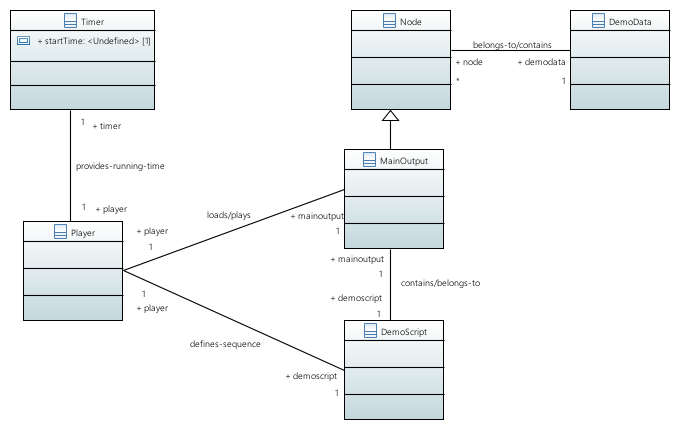
\includegraphics[width=0.8\textwidth]{img/player_domain_model.png}
    \caption{Domänenmodell der
        Player-Applikation\protect\footnotemark}\label{fig:domain-model:player}
\end{figure}
\footnotetext{Eigene Darstellung mittels Papyrus.}

Abbildung~\ref{fig:domain-model:player} zeigt das Domänenmodell der
Player-Applikation. Das Modell ist bewusst minimal gehalten und zeigt nur die
nötigsten Komponenten. Im Zentrum steht das Player-Objekt. Dieses liest ein
DemoScript, welches eine exportiert Echtzeit-Animation des Editors darstellt.
Ausgehend vom DemoScript kann schliesslich der Hauptknoten des Graphen gefunden
evaluiert werden. Ausgehend von diesem wird so die gesamte Echtzeit-Animation
aufgebaut und wiedergeben.

Viele essentielle Konzepte beziehungsweise Objekte fehlen in diesem Modell
bewusst. Diese werden während den Iterationen der darauffolgenden Projektarbeit
erarbeitet. Ein Teil davon findet sich im Domänenmodell des Editors
(\ref{subsec:domain-model:editor}) sowie im Klassendiagramm des Prototypen
(\ref{chap:prototype}).

\subsection{Editor}
\label{subsec:domain-model:editor}

\begin{figure}[H]
    \centering
    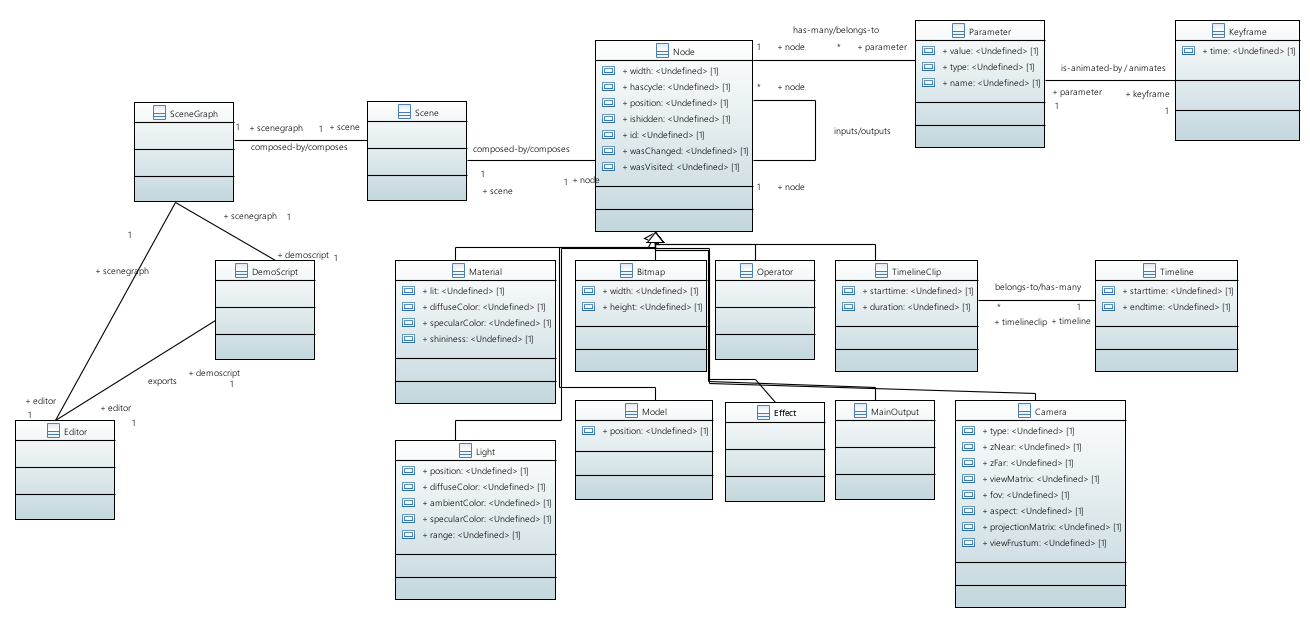
\includegraphics[angle=90,width=0.6\textwidth]{img/editor_domain_model.png}
    \caption{Domänenmodell der
        Editor-Applikation\protect\footnotemark}\label{fig:domain-model:editor}
\end{figure}
\footnotetext{Eigene Darstellung mittels Papyrus.}

Abbildung~\ref{fig:domain-model:editor} zeigt das Domänenmodell der
Editor-Applikation. Analog dem vorherigen Modell steht hier das Editor-Objekt
im Zentrum. Dieses bildet die Schnittstelle zwischen der grafischen
Benutzeroberfläche (GUI) und der Applikationslogik.

Die Komponenten der grafischen Benutzeroberfläche wurden in diesem Modell
bewusst weggelassen, da dies das Modell nur unnötig vergrössern würde. Die
eigentliche Logik findet sich in den essentiellen Konzepten beziehungsweise in
den hier gezeigten Objekten. Die grafische Benutzeroberfläche bildet diese nur
ab respektive Kopien davon.

Im mittleren Teil ist mit dem Node-Objekt und dessen Spezialisierung die
gesamte Struktur des Graphen angedeutet. Dies werden schliesslich die Objekte
sein, welche ein Anwender nutzen kann um Echtzeit-Animationen zu erstellen.

Im rechten Teil des Modelles stellen die Objekte Parameter, Keyframe,
TimelineClip und Timeline Elemente zur Animation dar. Pro Parameter kann zu
einem bestimmten Zeitpunkt der Zeitachse ein Schlüsselbild (Keyframe) gesetzt
werden. Timeline stellt die gesamte Zeitachse und TimelineClip einzelne
Elemente dieser dar. Es handelt sich bei Letzteren um Szenen.

Auch hier fehlen wiederum etliche Details, wie zum Beispiel das gesamte
Rendering inklusive den Shadern. Ein Teil davon ist wiederum im Klassendiagramm
des Prototypen (\ref{chap:prototype}) ersichtlich.

Wie Eingangs erwähnt, ist es nicht das Ziel ein vollständiges oder
``korrektes'' Domänenmodell zu erstellen. Es geht viel mehr um einen ersten
Anstoss zur eigentlichen Implementierung. Alle weiteren Details werden während
den Iterationen der darauffolgenden Projektarbeit erarbeitet.

% -*- coding: UTF-8 -*-
% vim: autoindent expandtab tabstop=4 sw=4 sts=4 filetype=tex
% vim: spelllang=de spell
% chktex-file 27 - disable warning about missing include files

\section{Sequenz-Diagramme}
\label{sec:sequence-diagrams}

Gemäss~\cite{larman_applying_2004} stellen Sequenz-Diagramme Ereignisse, welche
externe Akteure auslösen bzw.\ generieren, deren Ablauf sowie Ereignisse
zwischen Systemen eines spezifischen Szenarios eines Use Cases dar.

Da Sequenz-Diagramme schnell eine gewisse Grösse und auch Komplexität annehmen
wird in dieser Projektarbeit darauf verzichtet ein Sequenz-Diagramm für alle
Use Cases zu erstellen. Gerade bei \```UC2: Erstellen einer
Echtzeit-Animation\''' würde dies ansonsten grosse Ausmasse annehmen. Bei
Bedarf können diese bei den einzelnen Iterationen bzw.\ Phasen (Elaboration,
Construction und Transition). An dieser Stelle wird daher nur das
Sequenz-Diagramm für den ersten Use Case, \```UC1: Betrachten einer
Echtzeit-Animation\''' dargestellt. Dies deckt bereits einen Teil des Editors
mit ab.

\begin{figure}[H]
    \centering
    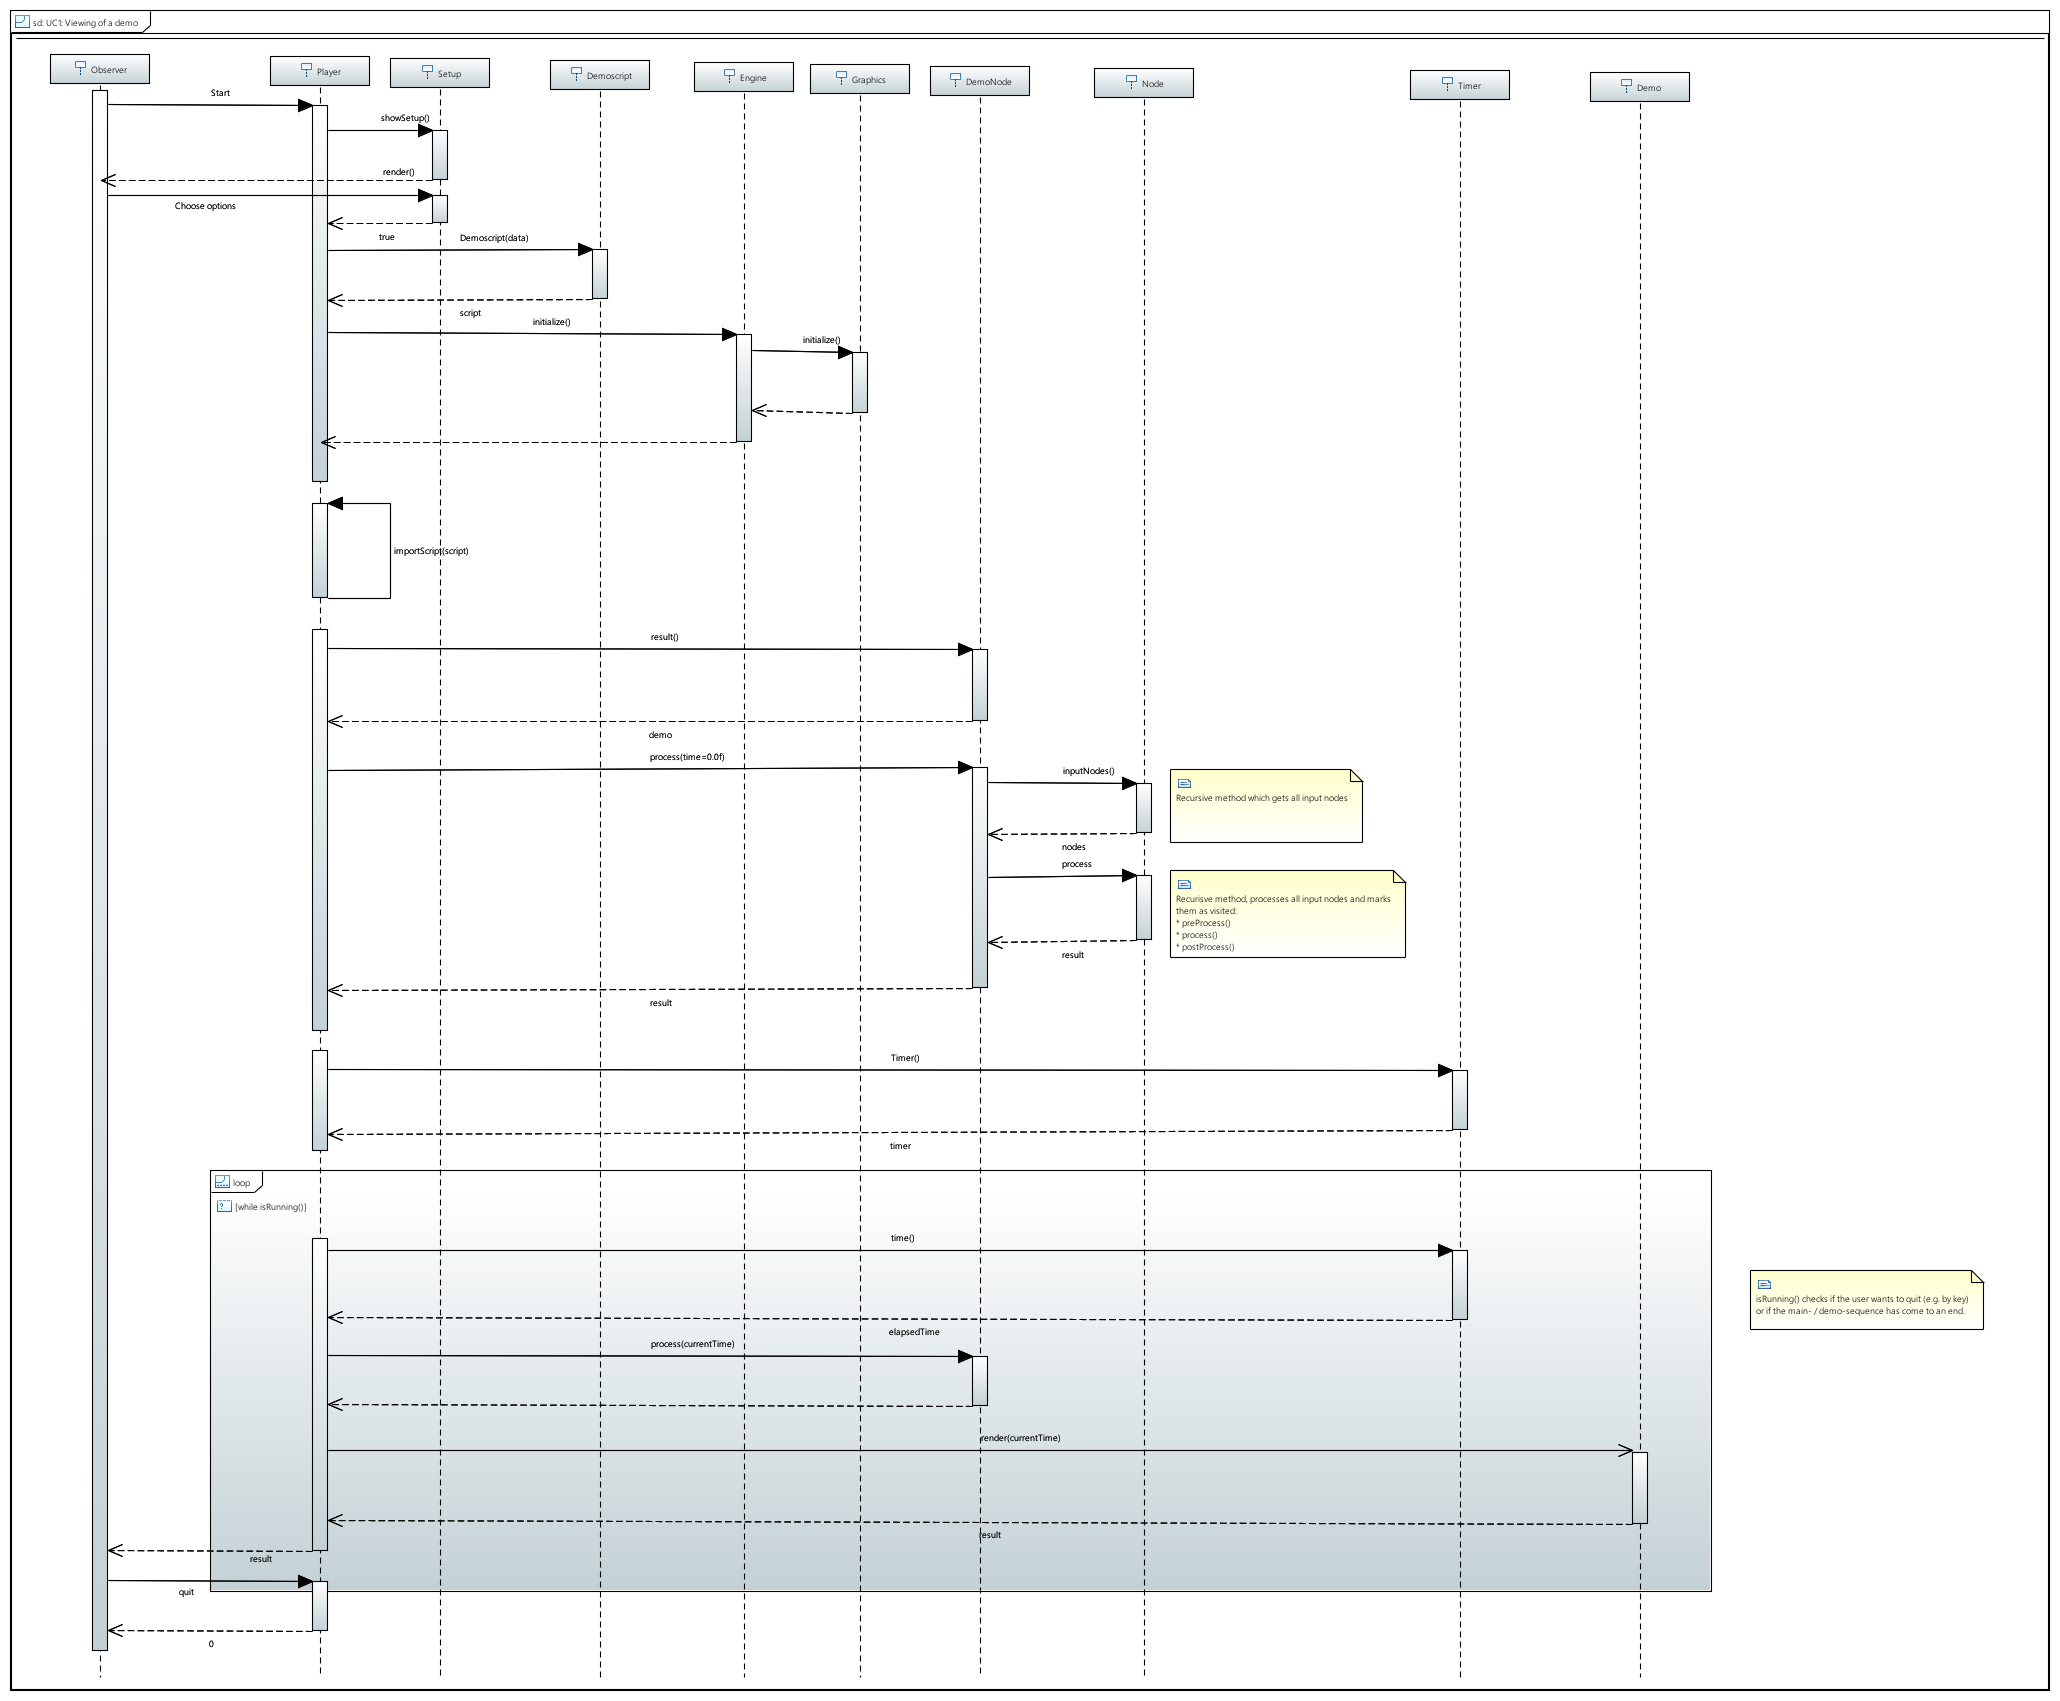
\includegraphics[angle=90,width=0.9\textwidth]{img/sequence_diagram_uc1.pdf}
    \caption{Sequenz-Diagramm  des Use Cases UC1
        \protect\footnotemark}\label{fig:package-diagram:editor}
\end{figure}
\footnotetext{Eigene Darstellung mittels Papyrus.}

\todo[inline]{Describe sequence diagram.}

% -*- coding: UTF-8 -*-
% vim: autoindent expandtab tabstop=4 sw=4 sts=4 filetype=tex
% vim: spelllang=de spell
% chktex-file 27 - disable warning about missing include files

\section{Logische Architektur}
\label{sec:logical-architecture}

Die logische Architektur zeigt das Gesamtbild der Software-Klassen in Form von
Paketen (bzw. Namespaces), Subsystemen und Layern~\cite{larman_applying_2004}.
Bei Layern handelt es sich um eine grobe Gruppierung von Klassen, Paketen oder
Subsystemen, welche zusammenhängen~\cite{larman_applying_2004}.

\subsection{Player}
\label{subsec:package-diagram:player}

\begin{figure}[H]
    \centering
    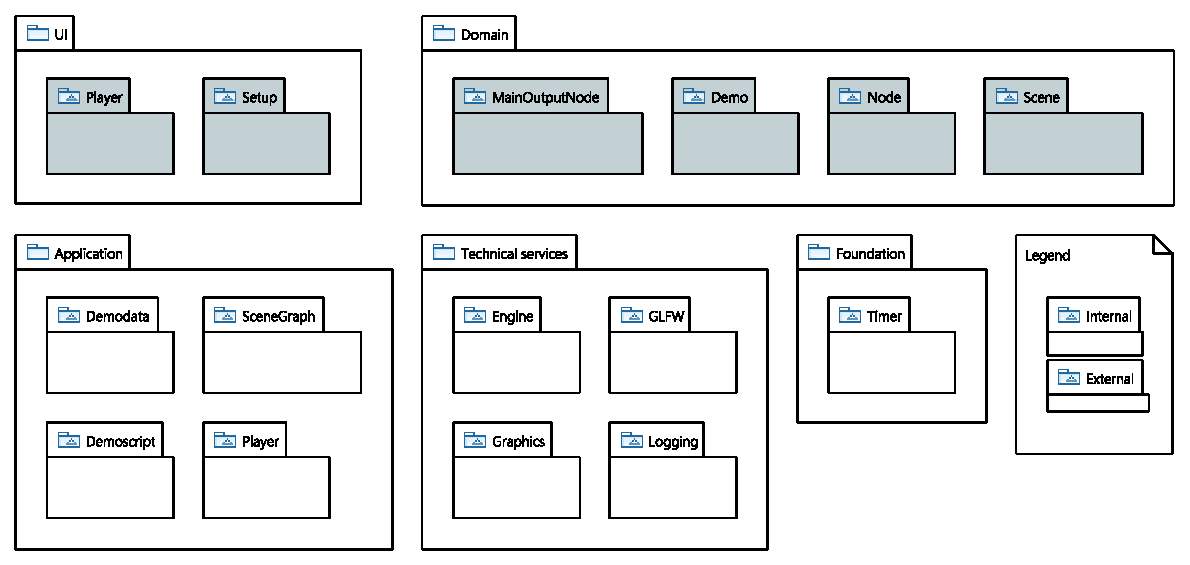
\includegraphics[width=0.7\textwidth]{img/player_package_diagram.pdf}
    \caption{Paket-Diagramm der
        Player-Applikation\protect\footnotemark}\label{fig:package-diagram:player}
\end{figure}
\footnotetext{Eigene Darstellung mittels Papyrus.}

\todo[inline]{Describe player package diagram.}

\subsection{Editor}
\label{subsec:package-diagram:editor}

\begin{figure}[H]
    \centering
    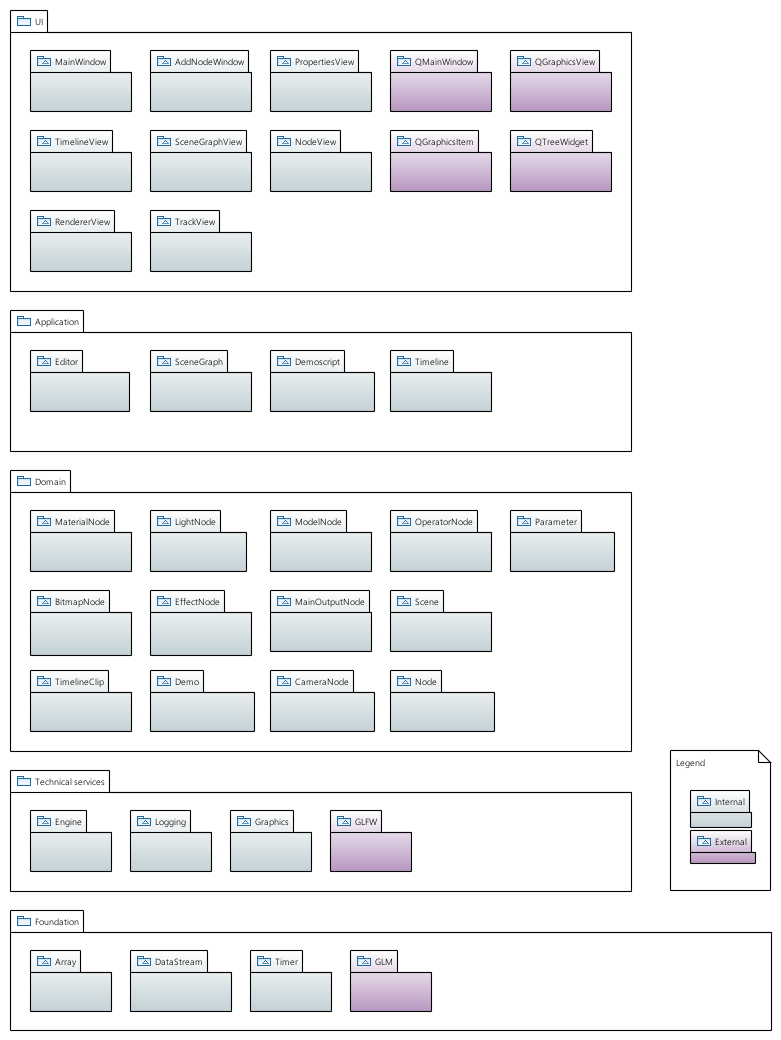
\includegraphics[width=0.9\textwidth]{img/editor_package_diagram.pdf}
    \caption{Paket-Diagramm der
        Editor-Applikation\protect\footnotemark}\label{fig:package-diagram:editor}
\end{figure}
\footnotetext{Eigene Darstellung mittels Papyrus.}

\todo[inline]{Describe editor package diagram.}


% -*- coding: UTF-8 -*-
% vim: autoindent expandtab tabstop=4 sw=4 sts=4 filetype=tex
% vim: spelllang=de spell
% chktex-file 27 - disable warning about missing include files

\chapter{Prototyp}
\label{chap:prototype}

Nach dem Finden und Ausarbeiten der Vision
(siehe~\autoref{subsec:requirements:vision}) sowie der Identifikation der
wichtigsten Komponenten (siehe~\autoref{sec:main-components}), wurde ein
Prototyp von Teilen der geplanten Software umgesetzt. Dies diente auch der
Identifikation der zusätzlichen Anforderungen
(siehe~\autoref{subsec:requirements:additional-requirements}).

Der Prototyp erlaubt die Modellierung einer einfachen Szene, bestehend aus
Primitiven, anhand der Graph-Komponente. Die Primitiven befinden sich in
externen (Shader-) Dateien, welche zur Laufzeit zusammen mit einem Haupt-Shader
geladen und zur Verfügung gestellt werden. Die nachfolgende Auflistung zeigt
die möglichen Unterverzeichnisse und Datei-Typen.

\begin{itemize}
    \item \textbf{data/objects/*.fs.xml}\\
        Sämtliche Objekt-Definitionen, wie zum Beispiel Kugel oder Würfel.
    \item \textbf{data/operations/*.fs.xml}\\
        Sämtliche Operationen, wie zum Beispiel die Vereinigung von Objekten.
    \item \textbf{data/misc/*.fs.xml}\\
        Diverse andere Definitionen, wie zum Beispiel Kameras.
    \item \textbf{data/sphere\_tracer.fs}\\
        Die Haupt-Shader-Datei, welche um Objekte, Operationen oder andere
        Definitionen ergänzt wird.
\end{itemize}

Durch die Modellierung wird der Haupt-Shader um Teile ergänzt und neu kompiliert, dies geschieht alles zur
Laufzeit in Echtzeit. Die Darstellung findet schliesslich mittels dem als
Sphere-Tracing bekannten Ray-Tracing-Verfahren
statt.~\autoref{listing:prototype:objects:sphere}
und~\autoref{listing:prototype:operations:union} zeigen Beispiel von
Shader-Defintionen.

\begin{minipage}{\linewidth}
\begin{lstlisting}[language=XML,caption={Objekt-Definition einer Kugel
        in XML.},label={listing:prototype:objects:sphere},captionpos=b,emph={xmlns,version,type}]
<?xml version="1.0" encoding="UTF-8"?>
<function>
    <name>sphere</name>
    <return-type>float</return-type>
    <parameters>
        <parameter>
            <name>position</name>
            <builtin>vec3</builtin>
            <type>property</type>
            <call>position - {}</call>
        </parameter>
        <parameter>
            <name>radius</name>
            <builtin>float</builtin>
            <type>property</type>
            <call>{}</call>
        </parameter>
    </parameters>
    <source>
        // Returns the signed distance to a sphere with given radius for the
        // given position.
        float sphere(vec3 position, float radius)
        {
            return length(position) - radius;
        }
    </source>
</function>
\end{lstlisting}
\end{minipage}

\begin{minipage}{\linewidth}
\begin{lstlisting}[language=XML,caption={Definition des Vereinigungs-Operators
        in XML.},label={listing:prototype:operations:union},captionpos=b,emph={castRay}]
<?xml version="1.0" encoding="UTF-8"?>
<function>
    <name>opUnion</name>
    <return-type>float</return-type>
    <parameters>
        <parameter>
            <name>a</name>
            <builtin>float</builtin>
            <type>input</type>
            <call>{}</call>
        </parameter>
        <parameter>
            <name>b</name>
            <builtin>float</builtin>
            <type>input</type>
            <call>{}</call>
        </parameter>
    </parameters>
    <source>
        // Returns the signed distance for a merge of given signed
        // distance a and signed distance b.
        float opUnion(float a, float b)
        {
            return min(a, b);
        }
    </source>
</function>
\end{lstlisting}
\end{minipage}

% -*- coding: UTF-8 -*-
% vim: autoindent expandtab tabstop=4 sw=4 sts=4 filetype=tex
% vim: spelllang=de spell
% chktex-file 27 - disable warning about missing include files

\section{Vorgehen}
\label{sec:prototype:procedure}

Die Entwicklung des Prototypen war ein iterativer Prozess. Es wurden Teil-Ziele
definiert, welche dann etappenweise erarbeitet wurden.

Das erste Teil-Ziel war das Neu-Kompilieren von Shadern während der Laufzeit,
so dass Shader während der Laufzeit erweitert, neu geladen und dargestellt
werden können.

Als zweites Teil-Ziel wurde dynamisches Laden von Shader-Dateien ausgehend vom
Verzeichnis des Prototypen implementiert.

Als drittes Teil-Ziel wurden Shader in Form von Templates umgesetzt.  Mit
``Jinja2CppLight'' (TODO~\todo{add reference to Jinja2CppLight here}) wurde
schliesslich ein Template-System eingeführt, welches es erlaubt Shader als
Templates zu parsen und Sektionen entsprechend mit Sub-Templates respektive
Teil-Shadern zu ersetzen.  Dies ermöglicht es Teile von Shadern während der
Laufzeit anzupassen. Durch die Erkenntnisse des ersten Teil-Zieles konnte der
aus dem Template zusammen mit den Sub-Templates generierte Shader zur Laufzeit
geladen und ausgeführt werden.

Als viertes und letztes Teil-Ziel wurde ein Prototyp der Graph-Komponente
(siehe~\ref{ssubsec:main-components:editor:graph}) umgesetzt. Der Graph bietet
ein Kontext-Menü zum Hinzufügen und Entfernen von Knoten. Für jeden
eingelesenen Teil-Shader wird ein Eintrag im Kontext-Menü hinzugefügt, so dass
dieser schliesslich dem Graphen hinzugefügt werden kann. Der Graph verfügt
standardmässig immer über einen (Haupt-) Ausgangs-Knoten.

Jeder der Knoten verfügt entweder über mindestens einen Eingang oder über einen
Ausgang.  Zusätzliche Ein- beziehungsweise Ausgänge werden je nach Typ eines
Knotens automatisch, dynamisch erstellt. Die Eingänge des Haupt-Knotens sind
jedoch statisch. Dieser verfügt über eine Haupt-Schnittstelle sowie eine
Schnittstelle für einen Kamera-Knoten.

Bei jeder neuen Verbindung beziehungsweise bei jedem Trennen einer Verbindung
innerhalb des Graphen, wird dieser neu evaluiert und die (Shader-) Ausgabe neu
berechnet.

Das Rendering ist schliesslich die Berechnung der relevanten Matrizen, binden
des Shaders und setzen der benötigten Uniform-Variablen.
Abbildung~\ref{fig:prototype:procedure} zeigt den aktuellen Stand des
Prototypen.

\begin{figure}[H]
    \centering
    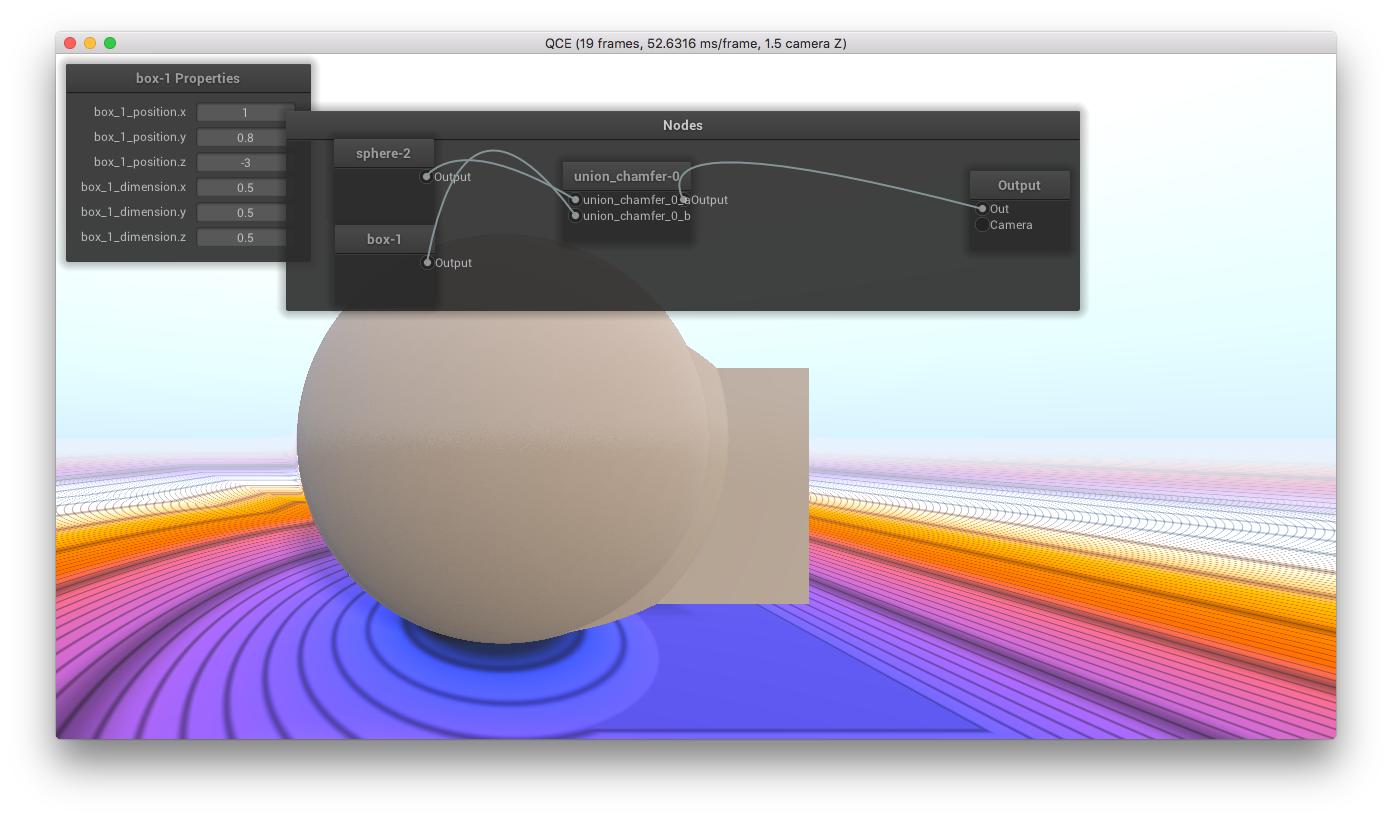
\includegraphics[width=0.9\textwidth]{img/prototype.png}
    \caption{Der Prototyp in Aktion
        \protect\footnotemark}\label{fig:prototype:procedure}
\end{figure}
\footnotetext{Eigene Darstellung.}

% -*- coding: UTF-8 -*-
% vim: autoindent expandtab tabstop=4 sw=4 sts=4 filetype=tex
% vim: spelllang=de spell
% chktex-file 27 - disable warning about missing include files

\section{Domänenmodell und Klassendiagramm}
\label{sec:prototype:domain-model-class-diagram}

Für den Prototypen wurde nicht explizit ein Domänenmdodell festgehalten. Dieses
wurde anhand der Vision und der Komponenten erstellt. Überlegungen dazu flossen
direkt in das Domänenmodell der Software-Architektur ein
(siehe~\autoref{sec:domain-model}).

In Abbildung~\ref{fig:class-diagram:prototype} findet sich das Klassendiagramm
des Prototypen. Blau-graue Elemente stellen dabei selbst entwickelte Pakete,
violette Elemente externe Pakete von Drittpersonen dar. Es wird bewusst
nicht das vollständige Klassendiagramm mit allen Elementen abgebildet, da dies
nach Meinung des Autors zu unübersichtlich würde. Die gesamte Struktur ist dem
Programmcode des Prototypen zu entnehmen, welcher dieser Projektarbeit
beiliegt.

\begin{figure}[H]
    \centering
    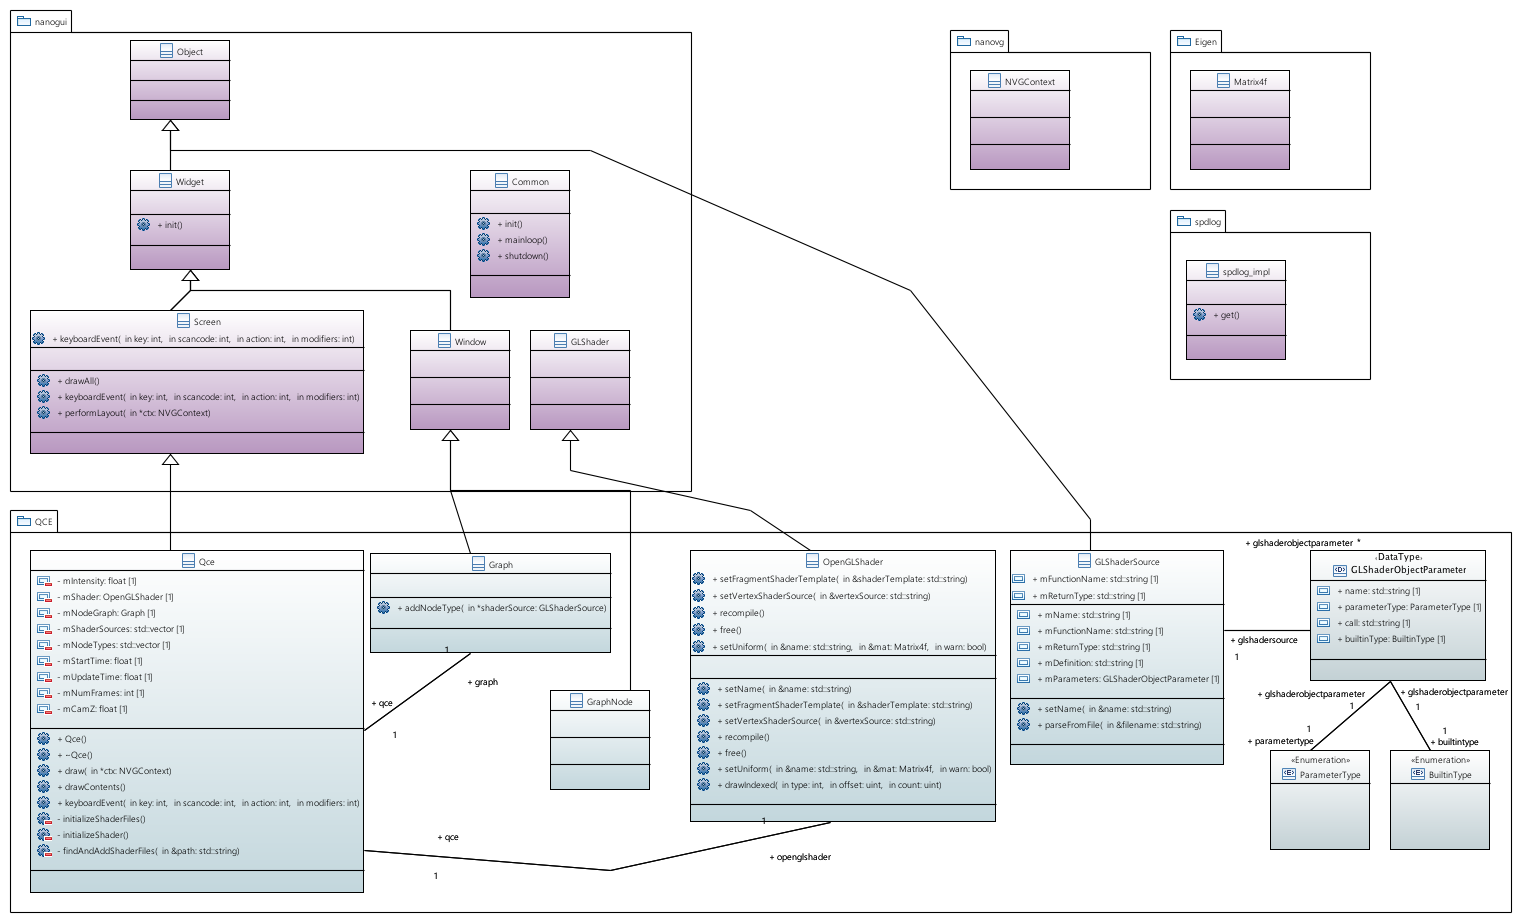
\includegraphics[angle=90,width=0.9\textwidth]{img/prototype_class_diagram.png}
    \caption{Klassendiagramm der Prototyp-Applikation}\label{fig:class-diagram:prototype}
\end{figure}

% -*- coding: UTF-8 -*-
% vim: autoindent expandtab tabstop=4 sw=4 sts=4 filetype=tex
% vim: spelllang=de spell
% chktex-file 27 - disable warning about missing include files

\section{Programmablauf}
\label{sec:prototype:sequence}

Nach dem Starten der Applikation erstellt diese die grafische
Benutzeroberfläche und lädt alle externen Shader-Dateien im Unterverzeichnis 
``data''. Die Haupt-Shader-Datei wird als Grundlage für den Ausgabe-Shader
genutzt, die Teil-Shader-Dateien bilden die wählbaren Objekte beziehungsweise
Einträge im Kontextmenü des Graphen.

Nach dem initialen Berechnen und Darstellen der Benutzeroberfläche befindet
sich die Applikation schliesslich in der Hauptschleife. Die Hauptschleife läuft
so lange bis der Benutzer diese mittels Tastendruck auf die Escape-Taste
unterbricht und damit die Applikation beendet.

In der Hauptschleife verarbeitet die Applikation diverse Events wie zum
Beispiel Maus- und Tastatur-Eingaben. Die Verarbeitung findet in der Regel
zuerst in den Kind-Klassen und dann schliesslich in der Hauptklasse statt. Dies
erlaubt es diversen Komponenten, welche eben Kind-Klassen der Applikation sind,
auf Ereignisse, wie zum Beispiel dem Erstellen einer Verbindung zwischen zwei
Knoten, zu reagieren.

Immer wenn ein Knoten dem Haupt-Ausgabeknoten des Graphen direkt oder indirekt
hinzugefügt wird, wird der Graph und somit der Shader neu berechnet
beziehungsweise kompiliert.

Beendet der Benutzer schliesslich die Hauptschleife via Druck auf die
Escape-Taste, so werden alle Ressourcen frei gegeben und die Applikation wird
beendet.

Eine vereinfachte Darstellung des Beschriebenen findet sich in
Abbildung~\ref{fig:prototype:sequence:activity}. Eine detailliertere
Darstellung findet sich in Abbildung~\ref{fig:prototype:sequence:diagram}.

\begin{figure}[H]
    \centering
    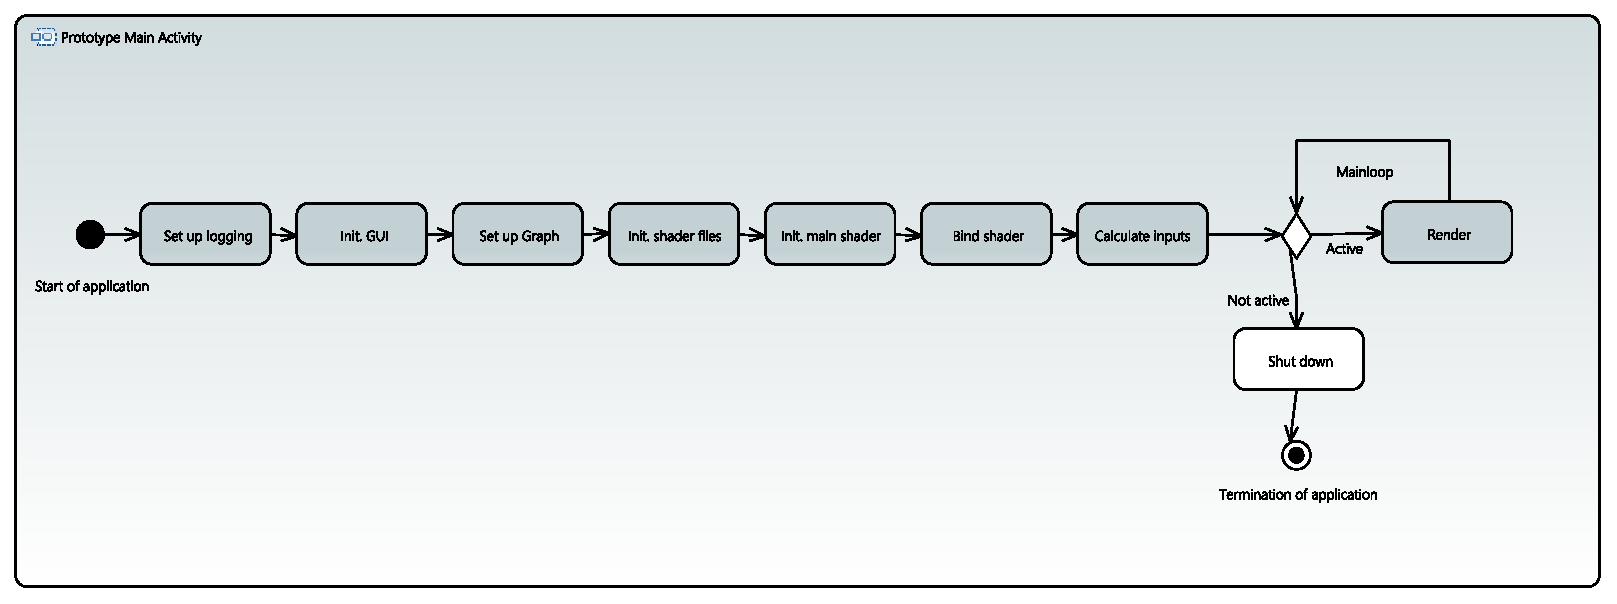
\includegraphics[width=0.9\textwidth]{img/prototype_activity_diagram.png}
    \caption{Vereinfachte Darstellung des Haupt-Programmablaufes
        \protect\footnotemark}\label{fig:prototype:sequence:activity}
\end{figure}
\footnotetext{Eigene Darstellung mittels Papyrus.}

\begin{figure}[H]
    \centering
    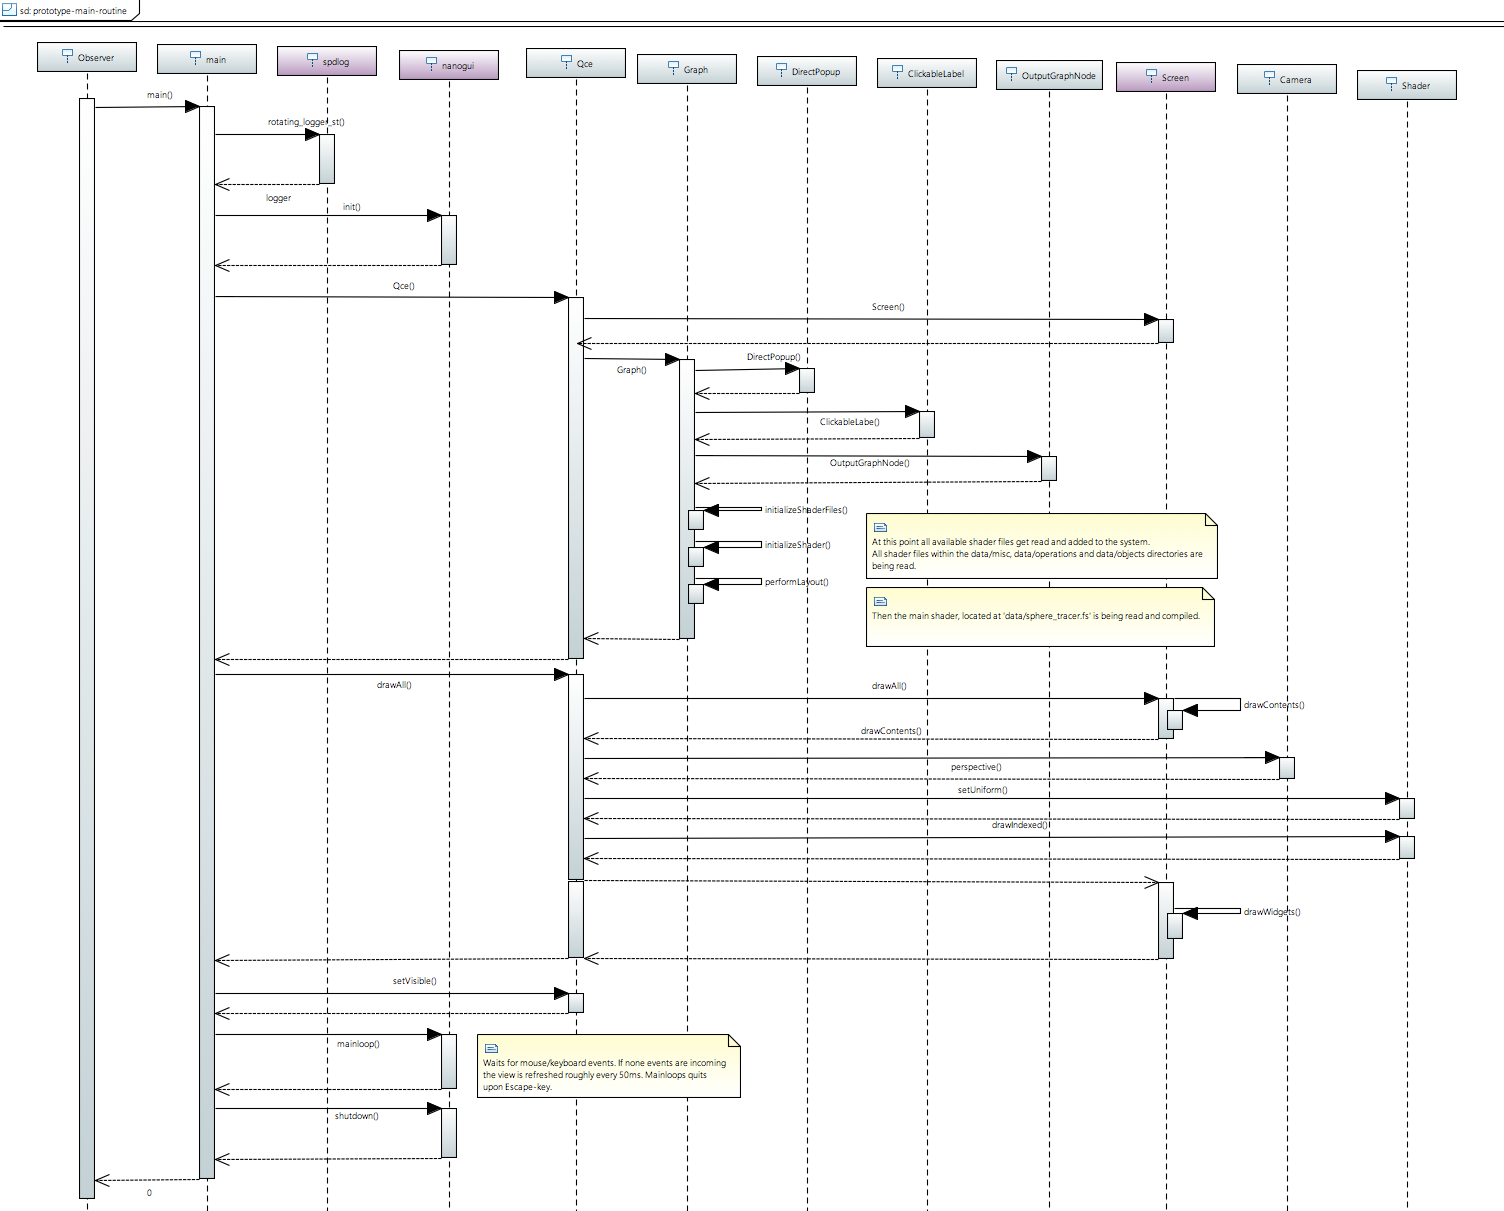
\includegraphics[width=0.9\textwidth]{img/prototype_sequence_diagram.png}
    \caption{Sequenz-Diagramm des Haupt-Ablaufes der
        Prototyp-Applikation\protect\footnotemark}\label{fig:prototype:sequence:diagram}
\end{figure}
\footnotetext{Eigene Darstellung mittels Papyrus.}

% -*- coding: UTF-8 -*-
% vim: autoindent expandtab tabstop=4 sw=4 sts=4 filetype=tex
% vim: spelllang=de spell
% chktex-file 27 - disable warning about missing include files

\section{Komponenten}
\label{sec:main-components}

Ausgehend von den Anforderungen (\ref{sec:requirements}) können einzelne
Komponenten der Applikation abgeleitet werden. Einzelne Teile davon wurden
schon durch die Vision (\ref{sec:vision}) definiert beziehungsweise aus dieser
gewonnen.

Dieser Prozess entspricht nicht direkt dem Vorgehen
gemäss~\cite{larman_applying_2004} beziehungsweise dem UP, der Autor dieser
Projektarbeit ist jedoch der Ansicht, dass dieser Abschnitt eine Brücke
zwischen Anforderungen und der (Software-) Modellierung bildet. Zudem bietet
dieser Abschnitt eine relativ bildliche Beschreibung, was dem Verständnis des
Gesamtkonzeptes sicher zuträglich ist. Am ehesten entspricht dieser Abschnitt
den Komponenten-Diagrammen in~\cite[S. 653 bis 654]{larman_applying_2004}.

Die Applikation besteht aus zwei Applikationen: Einem \textit{Player},
welcher dem Abspielen von Echtzeit-Animationen dient, sowie einem \textit{Editor},
welcher der Erstellung und Verwaltung von Echtzeit-Animationen dient.

\subsection{Player}
\label{subsec:main-components:player}

Der \textit{Player} liest die vom \textit{Editor} exportierten
Echtzeit-Animationen. Er bietet vor dem Abspielen die Auswahl der Auflösung,
des Seitenverhältnisses, Antialiasing und ob die Animation im Vollbild-Modus
abgespielt werden soll.

\subsection{Editor}
\label{subsec:main-components:editor}

Der \textit{Editor} erlaubt das Erstellen und Bearbeiten von
Echtzeit-Animationen. Diese können schliesslich inklusive den
dazugehörigen Dateien, wie zum Beispiel Bitmaps oder Modellen, exportiert
werden.

\begin{figure}[h]
    \centering
    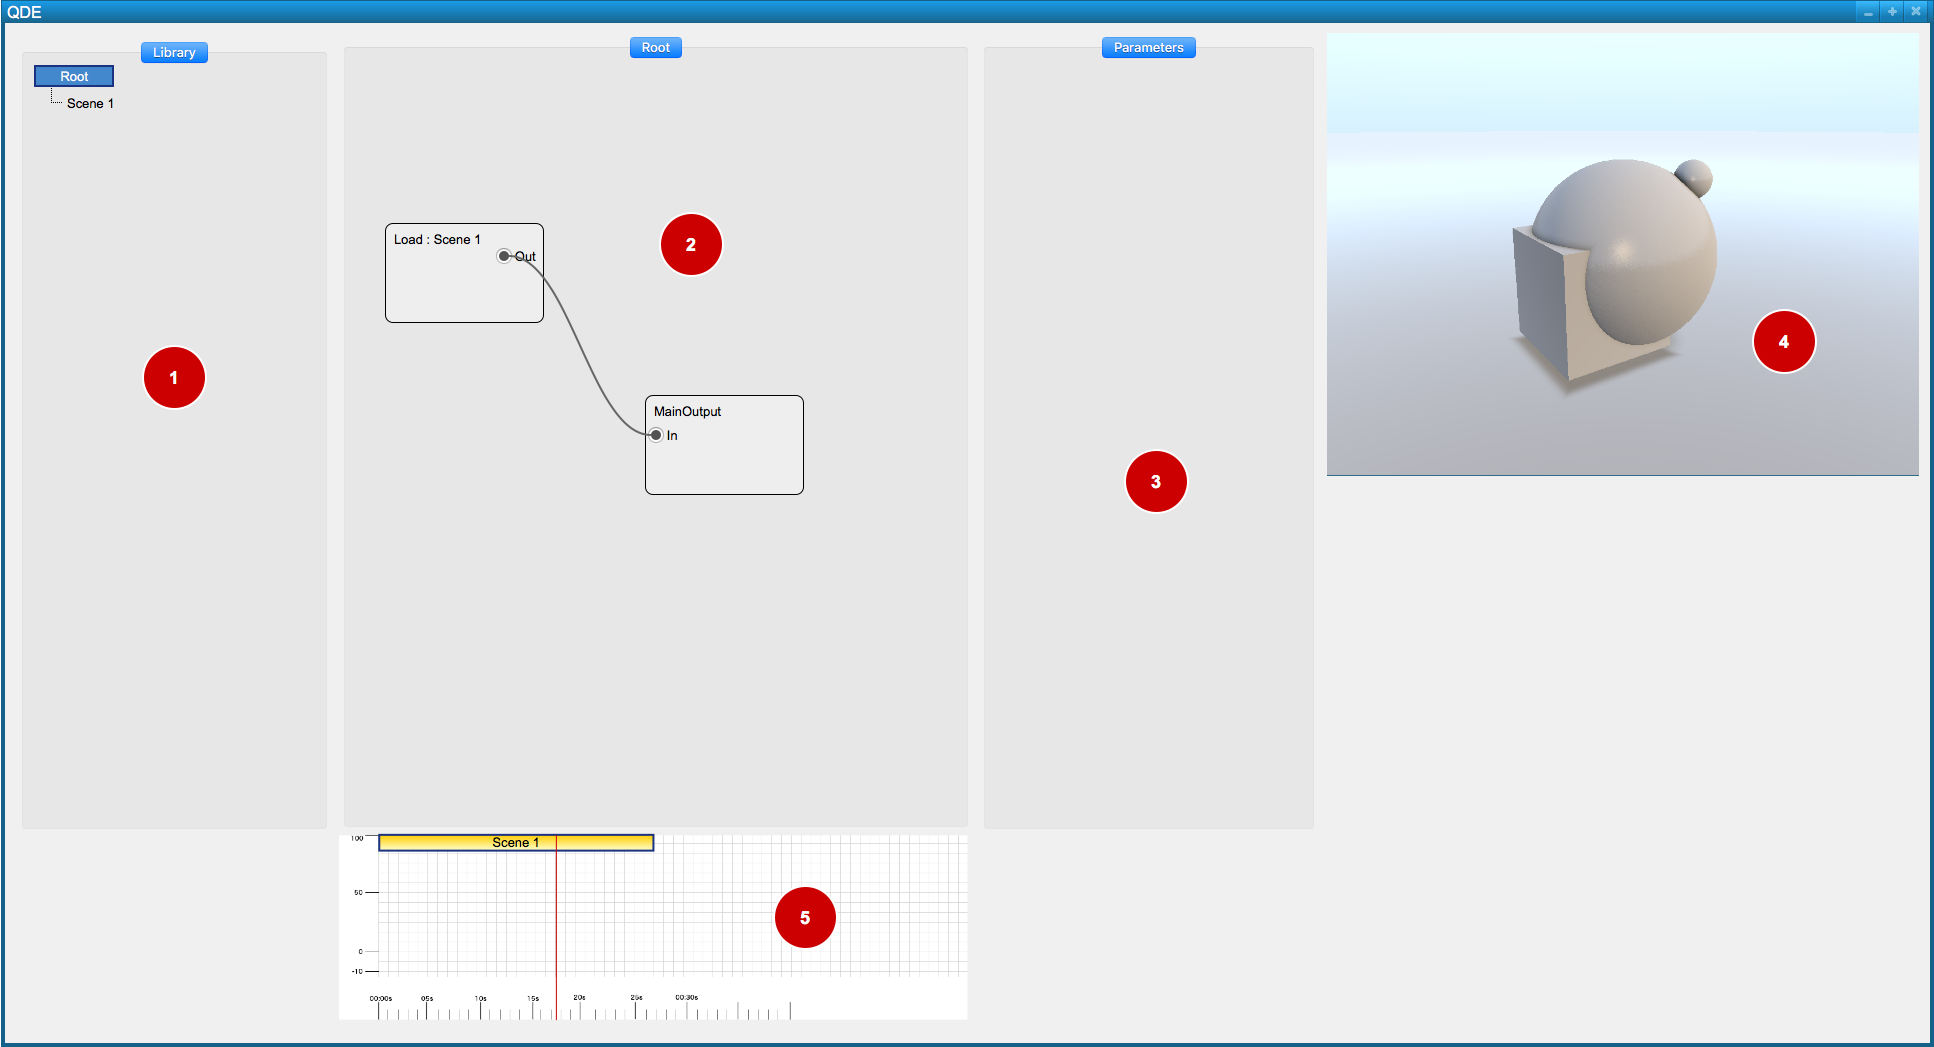
\includegraphics[width=0.9\textwidth]{img/editor_components.png}
    \caption{Einzelne Komponenten des Editors
        \protect\footnotemark}\label{fig:main-components:editor:editor-components}
\end{figure}
\footnotetext{Eigene Darstellung mittels Pencil.}

Abbildung~\ref{fig:main-components:editor:editor-components} zeigt die
einzelnen Komponenten des Editors. Nachfolgend findet sich eine Beschreibung
dieser.

\subsubsection{Bibliothek}
\label{ssubsec:main-components:editor:library}

Das Element~\img{img/editor_component_1.png} in
Abbildung~\ref{fig:main-components:editor:editor-components} zeigt die (Szenen-)
Bibliothek. Diese beinhaltet alle Szenen einer Echtzeit-Animation. Es können
neue Szenen angelegt und auch bestehende Szenen gelöscht werden. Wird ein neues
Projekt erstellt, so verfügt dieses immer über die ``Root''-Szene. Diese
beinhaltet den Haupt-Ausgabeknoten des Graphen
(\ref{ssubsec:main-components:editor:graph}), welcher schliesslich zum
Abspielen evaluiert wird, und kann nicht gelöscht werden. Wird eine Szene mit
der Maus angewählt, so wird deren Inhalt im Graphen
(\ref{ssubsec:main-components:editor:graph}) dargestellt.

\subsubsection{Graph}
\label{ssubsec:main-components:editor:graph}

Das Element~\img{img/editor_component_2.png} in
Abbildung~\ref{fig:main-components:editor:editor-components} zeigt den Graphen
einer Szene. Dieser beinhaltet sämtliche Knoten einer Szene. Mittels
Kontextmenü können neue Knoten eingefügt und bestehende Knoten gelöscht werden.
Wird ein Knoten angewählt, so wird dieser einerseits im
Rendering-Ansichtsfenster (\ref{ssubsec:main-components:editor:rendering})
dargestellt, andererseits werden dessen Eigenschaften im Parameter-Fenster
(\ref{ssubsec:main-components:editor:parameters}) angezeigt.

Folgende Typen von Knoten sind geplant:
\begin{itemize}
    \item{Scene}
    \item{TimelineClip}
    \item{Model}
    \item{Camera}
    \item{Light}
    \item{Material}
    \item{Operator}
    \item{Effect}
\end{itemize}

\subsubsection{Parameter}
\label{ssubsec:main-components:editor:parameters}

Das Element~\img{img/editor_component_3.png} in
Abbildung~\ref{fig:main-components:editor:editor-components} zeigt die Parameter
des aktuell gewählten Knoten im Graphen
(\ref{ssubsec:main-components:editor:graph}). Neben jedem Parameter befindet
sich eine Schaltfläche zum Setzen von Schlüsselbildern (Keyframes) in der
Zeitachse (Timeline,~\ref{ssubsec:main-components:editor:timeline}). Wird die
Schaltfläche betätigt, so wird bei dem aktuell ausgewählten Zeitpunkt der
Zeitachse ein Schlüsselbild gesetzt.

\subsubsection{Rendering}
\label{ssubsec:main-components:editor:rendering}

Das Element~\img{img/editor_component_4.png} in
Abbildung~\ref{fig:main-components:editor:editor-components} zeigt das
Rendering-Ansichtsfenster. Dieses stellt den Inhalt des aktuell gewählten
Knotens dar. Die Art des Knotens ist dabei nicht beschränkt, es kann dies eine
Szene, aber zum Beispiel auch ein einzelnes Modell sein. Es wird immer der
gesamte vorhergehende (Teil-) Baum des Knotens evaluiert.

\subsubsection{Zeitachse}
\label{ssubsec:main-components:editor:timeline}

Die Zeitachse wird mit~\img{img/editor_component_5.png} in
Abbildung~\ref{fig:main-components:editor:editor-scene1} dargestellt.  Sie
bildet das zeitliche Geschehen einer Echtzeit-Animation ab. Alle Knoten vom Typ
Timeline-Clip werden am oberen Rand des Fensters in deren zeitlicher
Reihenfolge abgebildet. Wird im Graph
(\ref{ssubsec:main-components:editor:graph}) ein Knoten mit animierten
Parametern (\ref{ssubsec:main-components:editor:parameters}) angewählt, so sind
diese ersichtlich. Vertikal wird der Wertebereich, horizontal die Zeitachse in
Sekunden dargestellt. Ein vertikal verlaufender, roter Marker zeigt die aktuelle
zeitliche Position der Echtzeit-Animation an.

Die untenstehende Abbildung~\ref{fig:main-components:editor:editor-scene1} zeigt ein Beispiel, wie eine typische Szene
mit animierten Parametern aussehen könnte.

\begin{figure}[H]
    \centering
    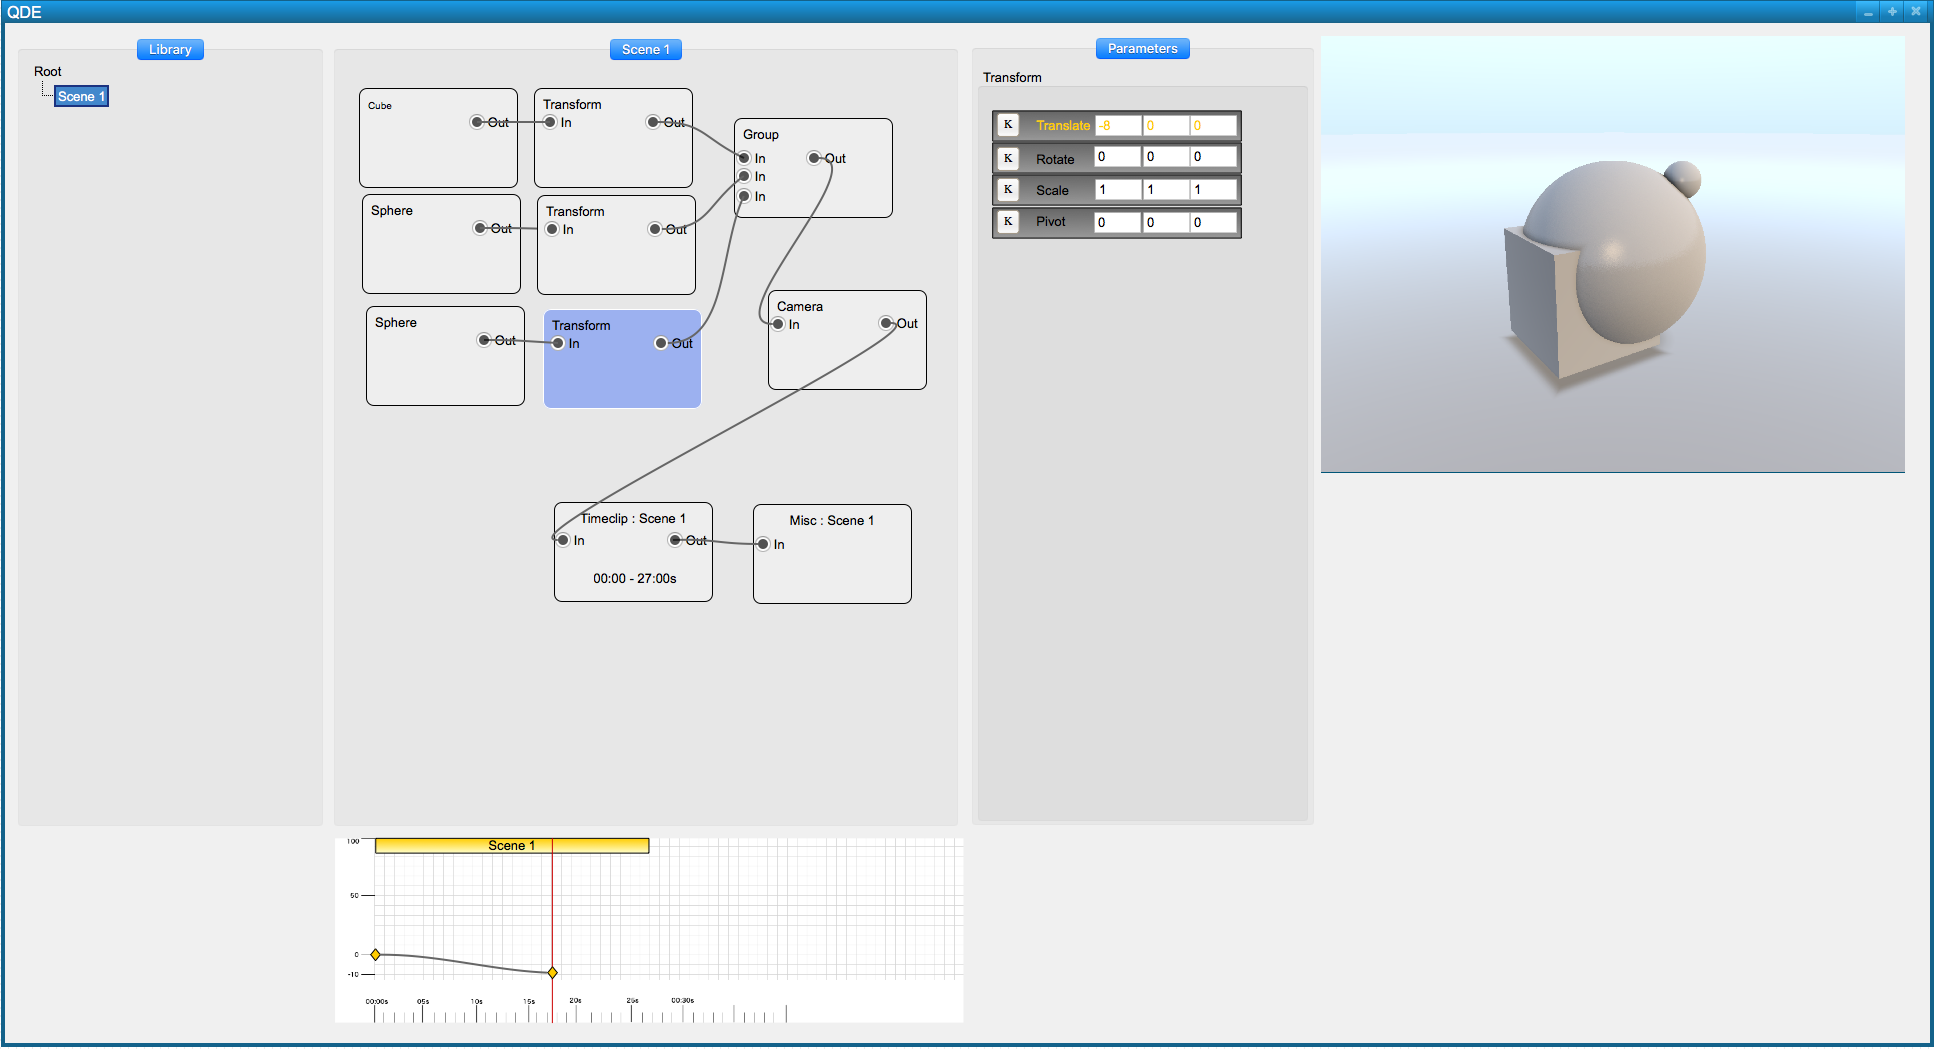
\includegraphics[width=0.9\textwidth]{img/editor_scene1.png}
    \caption{Beispiel-Szene innerhalb des Editors
        \protect\footnotemark}\label{fig:main-components:editor:editor-scene1}
\end{figure}
\footnotetext{Eigene Darstellung mittels Pencil.}

% -*- coding: UTF-8 -*-
% vim: autoindent expandtab tabstop=4 sw=4 sts=4 filetype=tex
% vim: spelllang=de spell
% chktex-file 27 - disable warning about missing include files

\section{Rendering}
\label{sec:prototype:rendering}

Auf das Rendering wird an dieser Stelle nicht näher eingegangen. Ein Teil wird
in~\autoref{sec:prototype:procedure} beschrieben. Der Rest findet sich im
nachfolgenden Kapitel über das verwendete Rendering, siehe~\autoref{chap:rendering}.


% -*- coding: UTF-8 -*-
% vim: autoindent expandtab tabstop=4 sw=4 sts=4 filetype=tex
% vim: spelllang=de spell
% chktex-file 27 - disable warning about missing include files

\chapter{Rendering}
\label{chap:rendering}


Um schliesslich die erstellte Echtzeit-Animationen auch darstellen zu können
--- im Editor und im Player --- wird ein Rendering-Verfahren benötigt.

Als Rendering-Verfahren soll primär das Ray-Tracing-Verfahren Sphere-Tracing
zum Einsatz kommen. Auf dieses wird hier nicht eingegangen, da dieses
bereits ausführlich in der vorhergehenden Projektarbeit behandelt wurde
(siehe~\ref{osterwalder_sven_volume_2016}).

Da bei der vorhergehenden Projektarbeit die~\textit{Berechnung von
    Normalen-Vektoren}, die \textit{Repetitions-Operation} und deren
\textit{Komplexität} nicht ausreichend geklärt wurden beziehungsweise bei der
Projektarbeit Fragen dazu aufkamen, werden die Punkte an dieser Stelle genauer
erläutert. Weiter wird ein möglicher Ansatz gezeigt, um \textit{herkömmliche
    3D-Modelle (Meshes)} mittels Sphere-Tracing darstellen zu können.

Als Grundlage für das Rendering wird OpenGL gewählt, da diese Bibliothek
plattformübergreifend und quelloffen ist. Mit der Einführung der Version 3 von
OpenGL, beziehungsweise Version 2 von OpenGL ES, wurde die Rendering-Pipeline
dahingehend geändert, dass diese nun nicht mehr fix vorgegeben sondern frei
programmierbar
ist\cite{opengl_foundation_fixed_2015}~\cite{opengl_foundation_rendering_2015}.
So gesehen findet das Rendering spätestens seit OpenGL Version 3
beziehungsweise OpenGL ES Version 2 immer per Shader statt. Ist der Aufwand der 
Programmierung der Rendering-Pipeline initial grösser, so ist eine frei
programmierbare Pipeline jedoch viel flexibler.

Genau dieser Ansatz soll auch in der hier vorgestellten Software-Architektur
für das Rendering verwendet werden: Ein modulares Rendering, welches jederzeit
ersetzt werden kann. Da alles via Shader gerendert wird, ist dies so gesehen
bereits gegeben. Szenen können --- im Falle von Sphere-Tracing --- rein aus
internen Funktionen und Daten bestehen oder aber --- im Falle der Verwendung
von herkömmlichen Modellen (Meshes) --- externe Daten beinhalten. So wäre
beispielsweise zusätzlich zu Sphere-Tracing
Deferred-Rendering~\footnotetext{https://sites.google.com/site/richgel99/home}~\parencite{saito_comprehensible_1990}
denkbar. Die Schnittstelle zwischen der Applikation und Shader, in Form von
Uniform-Variablen, wird aber so oder benötigt um auf der CPU berechnete
Matrizen an den Shader respektive die GPU weiterzureichen.

\section{Berechnung von Normalen-Vektoren}
\label{sec:rendering:normals}

Folgender Abschnitt basiert auf~\cite[S. 42 bis
43]{osterwalder_sven_volume_2016}.

Die Oberflächen-Normale kann gemäss~\citeauthor{hart_ray_1989} mittels dem
Gradienten des Distanzfeldes für einen bestimmten Punkt auf einer impliziten
Oberfläche berechnet werden~\parencite[S. 292 bis 293]{hart_ray_1989}.

Verwendet man dies nun zusammen mit den entsprechenden Distanzfunktionen, so
ergeben sich folgende Gleichungen:

\begin{gather}
    \bm{n}_{x} = f(x + \varepsilon, y, z) - f(x - \varepsilon, y, z) \\
    \bm{n}_{y} = f(x, y + \varepsilon,  z) - f(x, y - \varepsilon,  z) \\
    \bm{n}_{z} = f(x, y, z + \varepsilon) - f(x, y, z - \varepsilon) \\
\end{gather}

Dabei ist $\bm{n} = \begin{bmatrix} x_{n} \\ y_{n} \\ z_{n} \end{bmatrix}$ die
Normale der Oberfläche in Form eines Vektors mit drei Komponenten und $f$ eine
Distanzfunktion~\parencites[S. 292 bis 293]{hart_ray_1989}[S.
13]{hart_ray_1993}.

Es werden also insgesamt sechs Punkte abgetastet. $\varepsilon$ ist dabei ein
Wert um alle benachbarten Punkte eines gegebenen Punktes der impliziten
Oberfläche entlang der Koordinatenachsen zu erhalten. Da die Berechnung der
Normalen somit direkt von $\varepsilon$ abhängt, wird für $\varepsilon$
üblicherweise ein möglichst kleiner Wert verwendet.  \citeauthor{hart_ray_1989}
geben $\varepsilon$ als die minimale Inkrementation eines (Licht-) Strahles an.
Die Normale der Oberfläche sollte schliesslich noch normalisiert werden.

``Liefert die oben genannte Gradiente, bestehend aus 6 Punkten, eine zu
geringe Genauigkeit, so kann diese gemäss \citeauthor{hart_ray_1989}
erweitert werden~\parencite[S. 293]{hart_ray_1989}.\\
Die Erweiterung erfolgt durch Hinzunahme von Punkten, welche eine
gemeinsame Kante haben. Dies erzeugt eine Gradiente bestehend aus 18
Punkten. Werden noch die Punkte hinzugenommen, welche gemeinsame
Eckpunkte haben, so ergibt sich eine Gradiente bestehend aus 26
Punkten~\parencite[S. 293]{hart_ray_1989}.''~\cite[S.
43]{osterwalder_sven_volume_2016}

\section{Repetitions-Operation}
\label{sec:rendering:modulo}

Wie unter~\cite[S. 37ff]{osterwalder_sven_volume_2016} aufgeführt, existieren
für implizite Oberflächen diverse Operationen, wie Distanz- und
Domänen-Operationen sowie -Deformationen.

Möchte man nun aber dasselbe Objekt mehrmals darstellen, so repetiert man
dieses anhand einer oder mehrerer Achsen. Dies geschieht durch Anpassung der
Domäne, also der Anpassung des Raumes, in dem sich eine implizite Oberfläche
befindet. Es handelt sich dabei also um eine Domänen-Operation.

Die Anpassung der Domäne kann mittels der Modulo-Operation (mod, \%)
vorgenommen werden. Die Modulo-Operation gibt den (vorzeichenbehafteten) Rest
einer Division zurück~\cite{maignan_integer_2008}.

\begin{gather}
    d(\bm{x}, \bm{c}) = \bm{x} \mod \bm{c} - {\bm{c} \over 2}\\
    \text{repeat}(\bm{x}, \bm{c}) = f(d(\bm{x}, \bm{c}))
\end{gather}

Dabei ist $\bm{x}$ der Punkt einer impliziten Oberfläche $f$ und $\bm{c}$ der
gewünschte Abstand zwischen den Objekten.

Das Objekt wird erst mit der Hälfte des Abstandes $c$, also $c \over 2$, anhand
der Koordinatenachsen verschoben, um es im Rahmen des gewünschten Abstandes
$c$ zu zentrieren.  Danach wird die Repetition der Domäne angewendet. Danach
wird das Objekt zum Ursprung seines Koordinatensystemes zurück verschoben.

\subsection{Komplexität}
\label{subsec:rendering:modulo:complexity}

Es stellt sich nun die Frage, wie hoch die zusätzliche Komplexität bei
Anwendung der Modulo-Operation ist. Der Autor geht davon aus, dass der Aufwand
zur Darstellung von sich wiederholenden Objekten linear~\todo{is this correct?}
ist. Die Methode zum Abtasten der Distanz, \textit{castRay}, ändert sich in
diesem Sinne linear mit der Anzahl Objekte, die dargestellt werden sollen. Je
mehr Objekte, desto höher der Aufwand. Nimmt man nun an, dass ein Objekt,
welches wiederum eine Komposition von mehreren Objekten sein kann, wiederholt
wird, so wird dennoch nach Erreichen der maximalen Anzahl Schritte oder der
maximalen Distanz abgebrochen, was linear ist. Vereinfacht gesagt wird
schliesslich pro Iteration nur zurückgegeben, ob auf ein Objekt getroffen wurde
oder nicht. Die Berechnung der Beleuchtung respektiv der Farbe einer Oberfläche
erhöht die Komplexität natürlich nochmals.
Die Thematik soll an dieser Stelle jedoch nicht weiter vertieft werden, da dies
den Rahmen dieser Projektarbeit deutlich sprengen würde.

\section{Meshes}
\label{sec:rendering:meshes}

Während der Präsentation der vorhergehenden Projektarbeit, MTE7101, kam die
Frage auf, ob es auch möglich ist ``konventionelle'' 3D-Modelle (Meshes) mittels
Sphere-Tracing darzustellen. Die Modellierung bei der Anwendung von Sphere-Tracing findet 
üblicherweise mittels Distanzfunktionen statt und ist daher rein Mathematisch.
Sphere-Tracing nutzt Distanzfunktionen und Distanzfelder zur Darstellung von
impliziten Oberflächen~\cite[S. 31]{osterwalder_sven_volume_2016}.

Betrachtet man nun aber Meshes genauer, so handelt es sich prinzipiell auch um
Tiefeninformationen --- wie bei einem Distanzfeld. Somit müsste es möglich sein
ein Distanzfeld aus einem Mesh zu erzeugen und in einer dreidimensionalen
Textur abzuspeichern. Dazu könnte ein dreidimensionales Raster erzeugt und das
Mesh darin abgelegt werden. Danach müsste man die Distanzwerte von jedem Punkt
des Rasters zur Oberfläche des Meshes in der dreidimensionalen Textur ablegen.
Das Distanzfeld wäre dann zwar initial nicht $\in \R^{3}$, wie für das
Sphere-Tracing benötigt, das Speichern in eine dreidimensionale Textur würde
die Werte jedoch dann wieder auf [0, 1] beschränken.

Dem Autor dieser Arbeit ist bisher kein solches Verfahren bekannt. Ob die oben
beschriebene Methode wirklich funktioniert und wie gut die Resultate wären
müsste ausprobiert werden.

% -*- coding: UTF-8 -*-
% vim: autoindent expandtab tabstop=4 sw=4 sts=4 filetype=tex
% vim: spelllang=de spell
% chktex-file 27 - disable warning about missing include files

\chapter{Schlusswort}
\label{chap:discussion_and_conclusion}

In dieser Projektarbeit wurde eine Software-Architektur für ein System zur
einfachen Erstellung und Handhabung visueller Szenen in Echtzeit vorgestellt.
Die Projektarbeit dient als Vorarbeit zur darauffolgenden Projektarbeit,
MTE7103.

Zuerst wurde die \textit{Vision} erarbeitet und festgehalten. Die vorgestellte
Software-Architektur soll schliesslich zu einer Software zur Verwaltung und
Darstellung von Echtzeit-Animationen führen. Dabei soll sie es Anwendern
erlauben Echtzeit-Animationen in intuitiver Weise zu erstellen.

Ausgehend von der Vision wurden die \textit{Akteure} bestimmt sowie \textit{Use
    Cases} definiert.  Die Use Cases 1 bis und mit 5 wurden bewusst eher grob
granular gehalten um einen Überblick über die gesamte Software zu geben.
Details finden sich in den Uses Cases 6 bis 10.

Aufgrund der Anforderungen und Erfahrungen des Autors wurde mögliche Software
zur späteren Umsetzung der Software als \textit{zusätzliche Anforderung}
festgehalten.  Ursprünglich sollte NanoGUI für die grafische Umsetzung genutzt
werden. Bei der Implementation des Prototypen zeigte sich jedoch, dass die
Bibliothek nur bedingt für die Anforderungen aus der Software-Architektur
geeignet ist.  Stattdessen wird nun Qt in Betracht gezogen, da dies den
Grossteil aller Anforderungen bereits abdeckt.

Ausgehend von den Anforderungen wurden einzelne \textit{Komponenten der
    Applikation} abgeleitet und bildlich dargestellt. Die Applikation besteht
aus zwei Applikationen: Einem Player, welcher dem Abspielen von
Echtzeit-Animationen dient, sowie einem Editor, welcher der Erstellung und
Verwaltung von Echtzeit-Animationen dient.

Durch das Festhalten der Anforderungen und dem Identifizieren der einzelnen
Komponenten wurde schliesslich das \textit{Domänenmodell} erstellt, welches die Domäne
mit ihren essentiellen Konzepten oder Objekten zeigt.

Um eine Vorstellung vom Ablauf der Applikationen zu erhalten, wurde der erste
Use Case, ``UC1: Betrachten einer Echtzeit-Animation'', als
\textit{Sequenz-Diagramm} dargestellt. Das Sequenz-Diagramm ist in diesem Sinne
nicht vollständig, da dies ansonsten zu komplex und unübersichtlich würde. Es
geht nur darum ein grundlegendes Verständnis der Applikationen zu entwickeln.

Die Architektur wurde dann weiter ausgearbeitet und schliesslich folgte daraus
eine locker abgestufte Architektur (relaxed layered architecture). Diese wurde
mittels \textit{Paket-Diagrammen} grafisch dargestellt.

Um nun noch einen Schritt weiter zu gehen und der eigentlichen Umsetzung näher
zu kommen, wurden \textit{Klassendiagramme} der Applikation erstellt.

Zu dem Domänenmodell, dem Sequenz-Diagramm, den Paket-Diagrammen und den
Klassendiagrammen ist zu sagen, dass bei diesen einige essentielle
Konzepte beziehungsweise Objekte bewusst fehlen. Aufgrund der Vorgehensweise
anhand des Unified Processes (UP) ist ein iteratives Arbeiten vorgesehen, da
der UP auf agilen Ansätzen basiert. Das Ziel dieser Arbeit war nicht eine
komplette und ``korrekte'' Architektur zu erstellen, welche sich direkt
umsetzen lässt. Vielmehr dient diese als Grundlage für die darauffolgende
Arbeit, MTE7013 --- ``Master Thesis''. Bei dieser sollen dann die Details in
einzelnen Iterationsschritten erarbeitet und festgehalten werden.

Um Erfahrungen hinsichtlich der Umsetzung sammeln zu können sowie Erkenntnisse
betreffend Software zu erhalten, wurde ein \textit{Prototyp} umgesetzt. Der
Prototyp deckt nicht die gesamte Architektur ab sondern demonstriert die
Konzepte einzelner Teile der Software-Architektur. Der Prototyp erlaubt die
Modellierung einer einfachen Szene, bestehend aus Primitiven, anhand der
Graph-Komponente. Die Primitiven befinden sich in externen (Shader-) Dateien,
welche zur Laufzeit zusammen mit einem Haupt-Shader geladen und zur Verfügung
gestellt werden. Durch die Modellierung wird der Haupt-Shader um Teile ergänzt
und neu kompiliert, dies geschieht alles zur Laufzeit in Echtzeit. Die
Darstellung findet schliesslich mittels dem als Sphere-Tracing bekannten
Ray-Tracing-Verfahren statt. Dieses wurde in der vorhergehenden Projektarbeit
vorgestellt (siehe~\cite{osterwalder_sven_volume_2016}).

Im letzen Abschnitt wurde näher auf das Rendering-Verfahren eingegangen. Zudem
wurde mit der Repetition eine weitere Operation für implizite Oberflächen
vorgestellt und deren Komplexität betrachtet. Schliesslich wurde eine
Möglichkeit in Betracht gezogen, wie herkömmliche 3D-Modelle (Meshes) via
Sphere-Tracing dargestellt werden können. Dass diese Möglichkeit funktioniert ist
nicht gegeben, es handelt sich lediglich um eine Idee.

Im Nachhinein betrachtet wurde in der ersten Hälfte der Projektarbeit viel Zeit
in den Prototypen investiert. Der Fokus lag anfangs primär darin einen
lauffähigen Prototypen zu erhalten, anstatt zuerst ein (Software-) Design zu
erstellen. Dies hatte schliesslich zur Folge, dass keine saubere Trennung (zum
Beispiel in Schichten) stattfand und der Code weniger erweiterbar und wartbar
wurde. Als Schlussfolgerung kann man sagen, dass auch bei iterativem Vorgehen
und der Erstellung von Prototypen zuerst zumindest eine minimale Dokumentation
zum Beispiel in Form von Domänenmodellen, Klassendiagrammen und
Sequenz-Diagrammen erstellt werden sollte.

%---------------------------------------------------------------------------

% Glossary
%---------------------------------------------------------------------------
\cleardoublepage{}
\phantomsection{}
\addcontentsline{toc}{chapter}{Glossar}
\renewcommand{\glossaryname}{Glossar}
\glsaddall{}
\printglossaries{}
%---------------------------------------------------------------------------

% Bibliography
%---------------------------------------------------------------------------
\cleardoublepage{}
\phantomsection{}
\addcontentsline{toc}{chapter}{Literaturverzeichnis}
\printbibliography{}
%---------------------------------------------------------------------------

% Listings
%---------------------------------------------------------------------------
%\cleardoublepage
\phantomsection{}
\addcontentsline{toc}{chapter}{Abbildungsverzeichnis}
\listoffigures
%\cleardoublepage
\phantomsection{}
\addcontentsline{toc}{chapter}{Tabellenverzeichnis}
\listoftables
%\cleardoublepage
\phantomsection{}
\addcontentsline{toc}{chapter}{Auflistungsverzeichnis}
\lstlistoflistings{}
%---------------------------------------------------------------------------

% Index
%---------------------------------------------------------------------------
%\cleardoublepage
%\phantomsection{}
%\addcontentsline{toc}{chapter}{Stichwortverzeichnis}
%\renewcommand{\indexname}{Stichwortverzeichnis}
%\printindex
%---------------------------------------------------------------------------

% Attachment:
%---------------------------------------------------------------------------
%\appendix
\settocdepth{section}
% -*- coding: UTF-8 -*-
% vim: autoindent expandtab tabstop=4 sw=4 sts=4 filetype=tex
% chktex-file 27

% In den Anhang fügen Sie ein:
%  * Details des Projektpans, falls vorhanden
%  * Resultate und Zwischenresultate in Funktion der Projektiterationen
%  * Pflichtenheft / Anforderungsspezifikation (Stand Ende dritter Woche)
%  * Angaben zum Projektrepository
%  * Sitzungsprotokolle, falls vorhanden
%  * Weiterführende Erläuterungen zu den verwendeten Technologien, falls nötig
%  * Benutzerhandbuch, falls vorhanden und sinnvoll, es hier aufzulisten
%  * Installations- und Betriebsdokument, falls vorhanden und sinnvoll, es hier aufzulisten
% Unterlassen Sie das Anfügen von Listings.

\appendix 
\begin{titlepage}
    \clearpage
    \vspace*{\fill}
    \begin{center}
        \begin{minipage}{.6\textwidth}
            \fontsize{26pt}{28pt}\selectfont
            \chapter*{Anhang}\label{chap:attachment}
            \addcontentsline{toc}{chapter}{Anhang}
        \end{minipage}
    \end{center}
    \vfill % equivalent to \vspace{\fill}
    \clearpage
\end{titlepage}

\newpage
 % -*- coding: UTF-8 -*-
% vim: autoindent expandtab tabstop=4 sw=4 sts=4 filetype=tex

\chapter{Meeting minutes}
\label{chap:10_meeting_minutes}

% \VerbatimInput[label=20150921]{inc/static/attachment/minutes/20150921.rst}
% \newpage
% \VerbatimInput[label=20151004]{inc/static/attachment/minutes/20151004.rst}
% \newpage
% \VerbatimInput[label=20151011]{inc/static/attachment/minutes/20151011.rst}
% \newpage
% \VerbatimInput[label=20151011]{inc/static/attachment/minutes/20151018.rst}
% \newpage
% \VerbatimInput[label=20151011]{inc/static/attachment/minutes/20151025.rst}
% \newpage
% \VerbatimInput[label=20151011]{inc/static/attachment/minutes/20151102.rst}
% \newpage
% \VerbatimInput[label=20151011]{inc/static/attachment/minutes/20151115.rst}
% \newpage
% \VerbatimInput[label=20151011]{inc/static/attachment/minutes/20151206.rst}
% \VerbatimInput[label=20151011]{inc/static/attachment/minutes/20160125.rst}



% \includepdfset{pagecommand={\thispagestyle{headings}}}
% \includepdf[pages=-, addtotoc={1,chapter,0,Anforderungsdokument,chap:anf},scale=0.95]{anhang/anforderungen.pdf}
% \newpage
% \includepdf[pages=-, addtotoc={1,chapter,0,Tutorial Wissensmodellierung,chap:tutorial},scale=0.95]{anhang/Tutorial.pdf}
% \newpage
% \input{anhang/schnipsel}
% \newpage
% \input{anhang/modellierung}
% \newpage
% \input{anhang/installationshandbuch}
% \newpage
% \includepdf[pages=-, addtotoc={1,chapter,0,Arbeitsjournal ,chap:arbeitsjournal},scale=0.95]{anhang/Journal.pdf}
% \newpage

%---------------------------------------------------------------------------

\end{document}
